\chapter{Risultati}

Negli scorsi due capitoli abbiamo presentato i metodi utilizzati per studiare numericamente l'evoluzione dei dischi circumstellari in sistemi binari.
Le caratteristiche del disco a cui siamo interessati sono due:
\begin{list}{\textbf{-}}{\setlength{\itemsep}{0cm}}
    \item le dimensioni dell'oggetto
    \item l'eccentricità delle orbite percorse dal materiale presente nell'intorno della regione di troncamento
\end{list}
Per questo motivo il seguente capitolo è organizzato in due macro-sezioni, ciascuna delle quali è dedicata ad uno dei due parametri a cui siamo interessati.
L'estensione del disco è trattata in Sezione \ref{sec:dim_disc}, mentre la \ref{sec:ecc_disc} è dedicata allo studio di $e_{disco}$.
L'ultima parte di questo capitolo è dedicata al confronto con le predizioni teoriche ottenute da \textcite{ManaraTronc2019} (vedi Sezione \ref{sec:fis_tronc})

\section{Dimensioni del disco} \label{sec:dim_disc}

Abbiamo determinato le estensioni dei dischi secondo due approcci differenti: il metodo dei raggi ed il metodo dei semiassi maggiori (vedi Sezione \ref{sec:metnum_anal}).
Le simulazioni effettuate sono tutte della lunghezza di 50 orbite del sistema binario: notiamo che dopo le prime 10 orbite, come in \textcite{ArtymowiczLubow1994} viene raggiunta una configurazione quasi-stabile, che varia lentamente al passare del tempo.
In accordo con quanto fatto da \textcite{ArtymowiczLubow1994}, i risultati che presentiamo nelle seguenti sottosezioni sono i valori di $r_T/a$ e $a_T/a$ mediati nel tempo dalla trentesima alla cinquantesima orbita del sistema binario: lavorando in questo modo otteniamo dei valori che non dipendono dalla singola configurazione del sistema, ma che invece fanno riferimento ad un suo comportamento medio.
I risultati ottenuti sono riportati in Appendice \ref{appendiceD}.

\subsection{Raggi di troncamento}

Le Figure \ref{fig:raggi_alfa2}, \ref{fig:raggi_alfa3}, \ref{fig:raggi_alfa4} riportano quanto abbiamo trovato per i raggi dei dischi nelle tre casistiche di viscosità analizzate. Sull'ascissa dei grafici è posto il rapporto $m_{cen}/m_{per}$, dove $m_{cen}$ indica la massa della stella posta al centro della griglia, mentre $m_{per}$ quella del corpo perturbante. Sulle ordinate è riportata l'eccentricità $e$ della binaria. 

\begin{figure}[H]
  \centering
  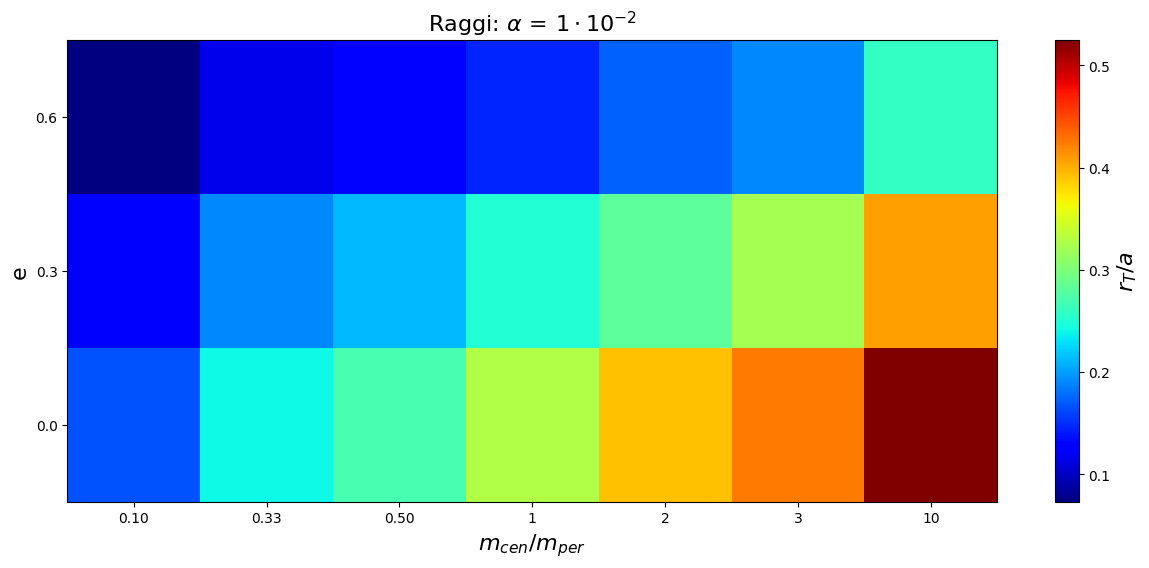
\includegraphics[width=\textwidth]{Immagini/Risultati/raggi_alfa2.png}
  \caption{Raggi di troncamento dei dischi circumstellari con $\alpha\,=\,1 \cdot 10^{-2}$. }
  \label{fig:raggi_alfa2}
\end{figure}

\begin{figure}[H]
  \centering
  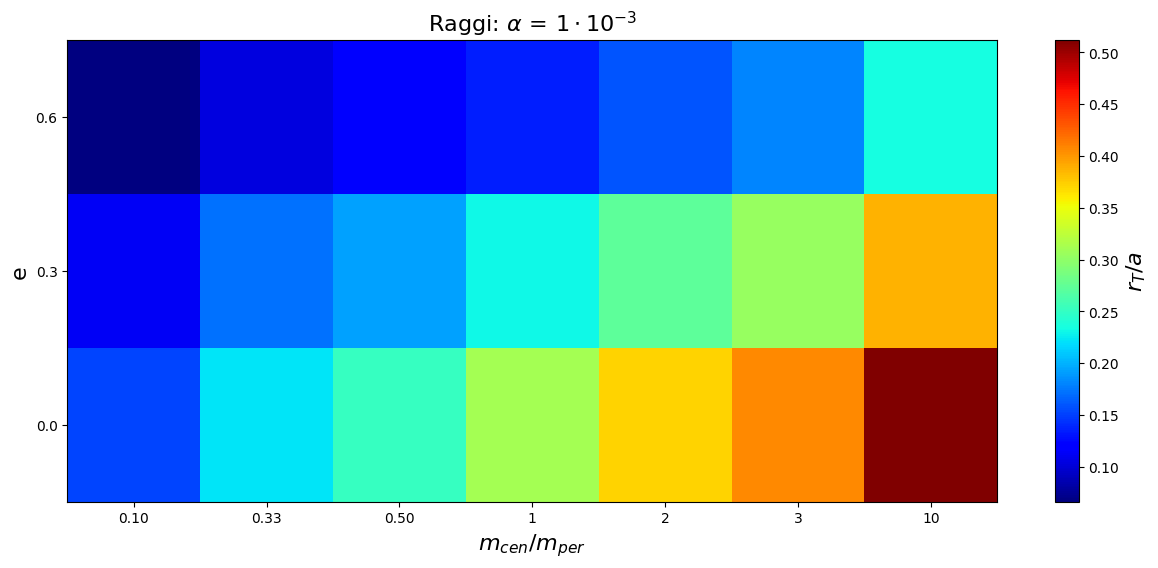
\includegraphics[width=\textwidth]{Immagini/Risultati/raggi_alfa3.png}
  \caption{Raggi di troncamento dei dischi circumstellari con $\alpha\,=\,1 \cdot 10^{-3}$}
  \label{fig:raggi_alfa3}
\end{figure}

\begin{figure}[h]
  \centering
  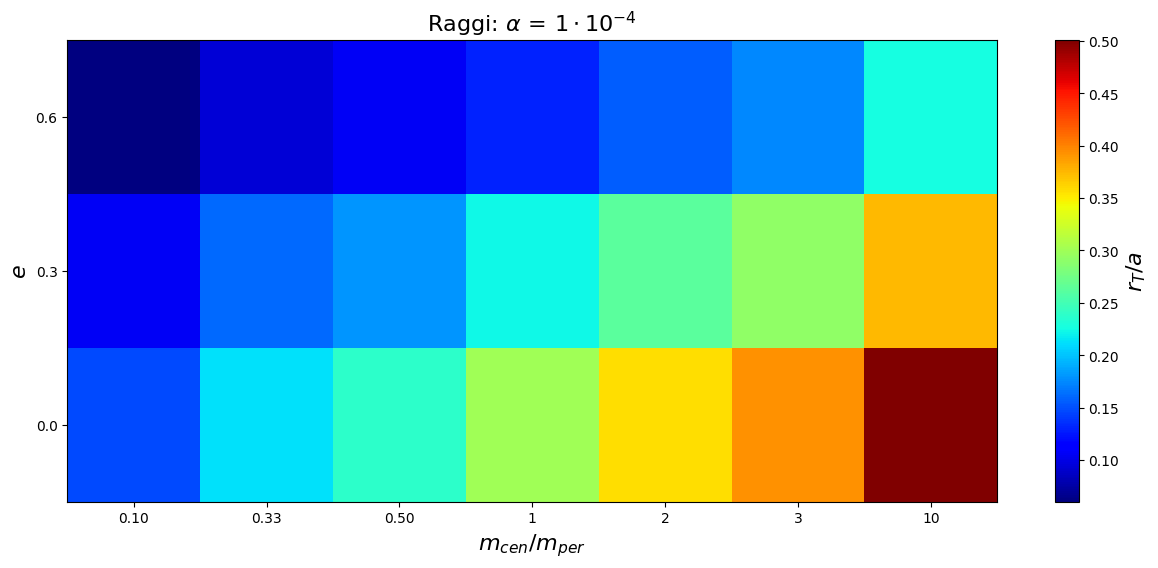
\includegraphics[width=\textwidth]{Immagini/Risultati/raggi_alfa4.png}
  \caption{Raggi di troncamento dei dischi circumstellari con $\alpha\,=\,1 \cdot 10^{-4}$}
  \label{fig:raggi_alfa4}
\end{figure}
La dimensione del disco ad $e$ ed $m_{cen}/m_{per}$ fissati è data dal colore della rispettiva cella nel grafico: la scala ha come estremi il valor minimo ed il valore massimo di $r_T$. 

Notiamo che ad eccentricità della binaria fissata, i valori maggiori di $r_T$ vengono assunti in corrispondenza di rapporti $m_{cen}/m_{per}$ elevati: questo accade poiché le dimensioni dei \textit{Roche Lobe} sono maggiori tanto più grande è la frazione della massa totale del sistema $M\,=\,m_{cen}\,+\,m_{per}$ contenuta al loro interno.
Nel caso di $m_{cen}/m_{per}\,=\,10$, sebbene il gas si trovi a $r/a \sim 0.5$, risulta ancora gravitazionalmente legato alla stella posta al centro della griglia simulativa.

Supponiamo ora di fissare $m_{cen}/m_{per}$ e di variare invece l'eccentricità della binaria: notiamo una netta diminuzione del valore assunto dal raggio del disco. All'aumentare di $e$, l'intensità delle risonanze eccentriche risulta essere più elevata \parencite{ArtymowiczLubow1994} e la regione in cui avviene il troncamento cambia.

Osserviamo anche una leggera dipendenza sulla viscosità del materiale costituente il disco: maggiore è $\alpha$, maggiori sono le dimensioni che vengono raggiunte dal corpo orbitante attorno alla stella. Tale andamento era noto in letteratura per i dischi ospitati in sistemi binari eccentrici, ma non per quanto riguarda quelli circolari. Nella seguente tabella riportiamo le massime e minime estensioni ottenute per i tre $\alpha$:

\begin{table}[H]
\centering
\begin{tabular}{|C{2cm}|C{3cm}|C{3cm}|C{3cm}|}
\hline
\rowcolor{yellow}
Tipo & $\alpha\,=\,1 \cdot 10^{-2}$ & $\alpha\,=\,1 \cdot 10^{-3}$ & $\alpha\,=\,1 \cdot 10^{-4}$\\
\hline
Maggiore & $0.525\,a$ & $0.512\,a$ & $0.501\,a$\\
\hline
Minore & $0.073\,a$ & $0.066\,a$ & $0.060\,a$\\
\hline
\end{tabular}
\end{table}

\newpage

\subsection{Semiassi di troncamento} \label{subsec:semiax_tr}

Nelle Figure \ref{fig:sax_alfa2}, \ref{fig:sax_alfa3}, \ref{fig:sax_alfa4} abbiamo riportato quanto ottenuto per i tre $\alpha$ analizzati: i grafici sono dello stesso tipo di quelli della sezione precedente.

\begin{figure}[H]
  \centering
  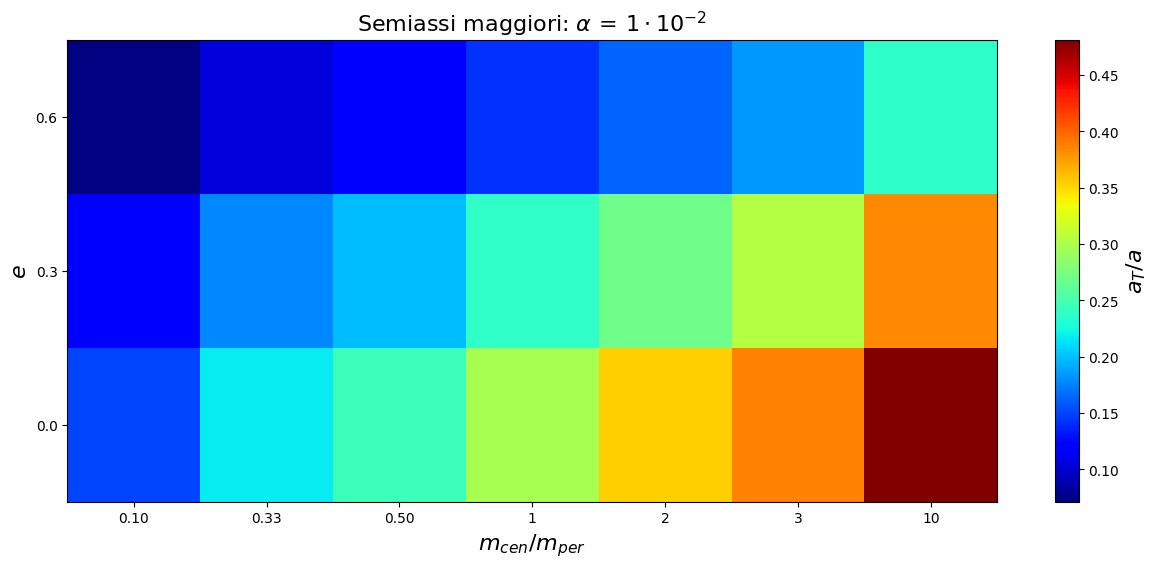
\includegraphics[width=\textwidth]{Immagini/Risultati/semiassi_alfa2.png}
  \caption{Semiassi maggiori dei dischi circumstellari con $\alpha\,=\,1 \cdot 10^{-2}$. }
  \label{fig:sax_alfa2}
\end{figure}

\begin{figure}[H]
  \centering
  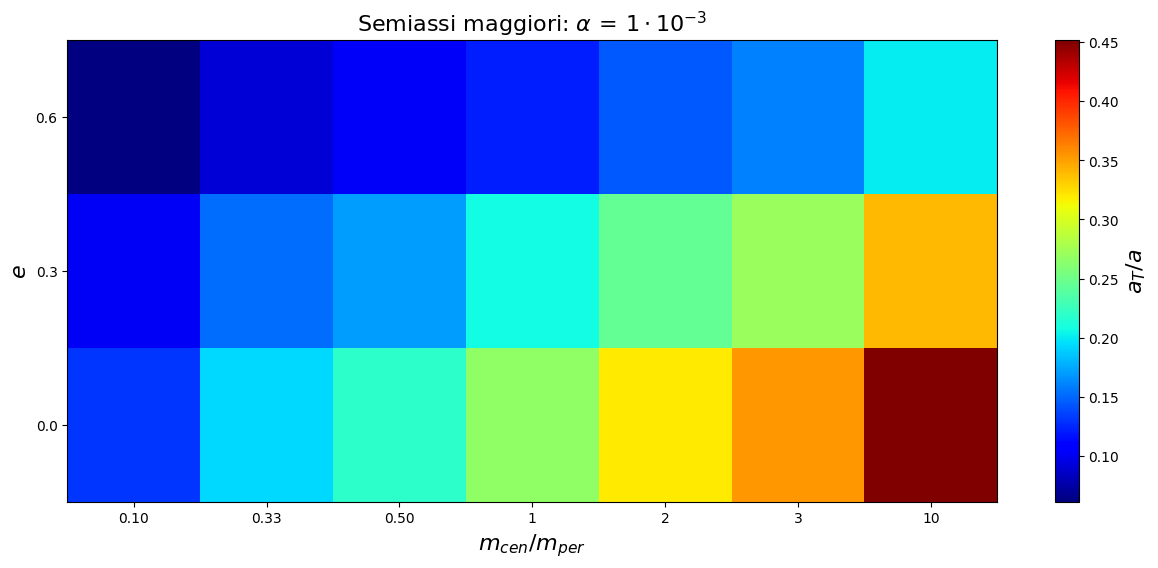
\includegraphics[width=\textwidth]{Immagini/Risultati/semiassi_alfa3.png}
  \caption{Semiassi maggiori dei dischi circumstellari con $\alpha\,=\,1 \cdot 10^{-3}$. }
  \label{fig:sax_alfa3}
\end{figure}

\begin{figure}[H]
  \centering
  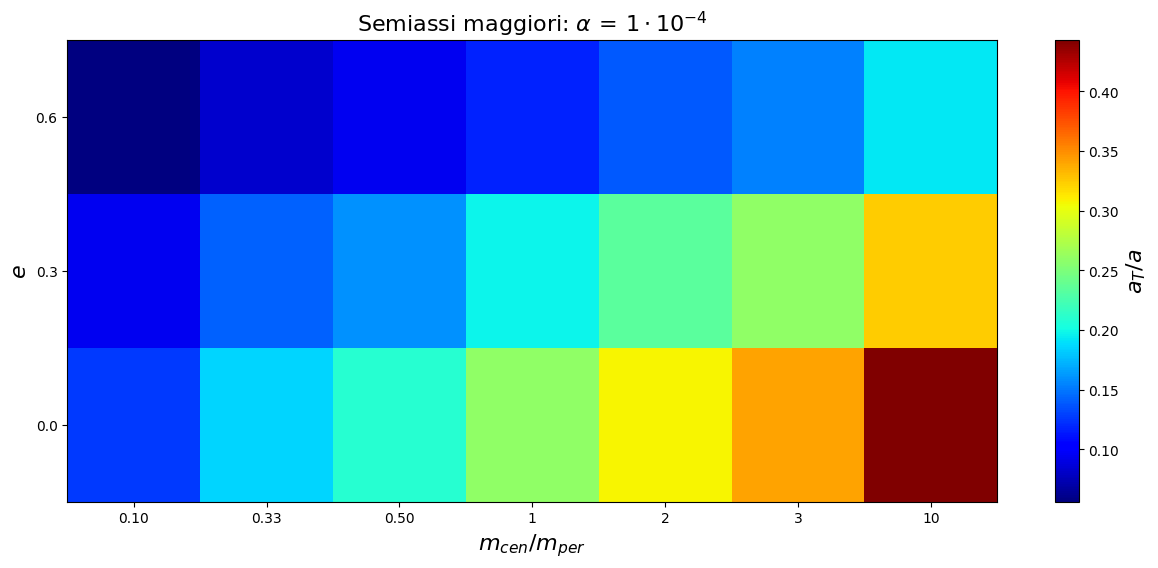
\includegraphics[width=\textwidth]{Immagini/Risultati/semiassi_alfa4.png}
  \caption{Semiassi maggiori dei dischi circumstellari con $\alpha\,=\,1 \cdot 10^{-4}$. }
  \label{fig:sax_alfa4}
\end{figure}
Osserviamo gli stessi andamenti presenti nel caso dei raggi di troncamento: il valore di $a_T/a$ è fortemente dipendente da $m_{cen}/m_{per}$ e dall'eccentricità della binaria.
Notiamo che anche per il metodo dei semiassi a valori più elevati di viscosità corrispondono estensioni spaziali dei dischi maggiori.\\

\textbf{Confronto con i raggi}\\

La necessità di lavorare in termini di semiasse maggiore del disco è evidenziata dalla Figura \ref{fig:moma_grid}: notiamo che a raggio fissato i valori di momento angolare specifico assunti nelle singole cellette spaziano un ampio intervallo.
Questa evidenza numerica non è in accordo con il modello di disco costituito da materiale orbitante lungo traiettorie circolari necessario per la determinazione di $r_T$.

Il metodo dei raggi di troncamento porta a una sovrastima delle effettive dimensioni del disco, poiché il materiale gassoso durante la sua orbita attorno alla stella spende più tempo ad apoastro: i valori di $a_T/a$ ottenuti sono inferiori rispetto a quelli di $r_T/a$. La discrepanza è dovuta al fatto che i dischi sono eccentrici: questa particolarità non è trascurabile.

La Figura \ref{fig:discr_disc} evidenzia come la differenza fra il metodo dei raggi e quello dei semiassi non sia trascurabile: dato che a seconda delle applicazioni si può essere interessati ad $a_T$ oppure ad $r_T$, è necessario tener conto delle loro differenze.
Sull'asse delle ascisse è posta la dimensione del semiasse, mentre su quello delle ordinate la variazione percentuale con il corrispondente valore di $r_T$.
Notiamo che la discrepanza fra i valori ottenuti con i due metodi oscilla fra il $10\%$ ed il $20\%$: questo accade poiché i dischi presentano delle eccentricità $e_{disco}$ che variano di caso in caso.

\begin{figure}[H]
  \centering
  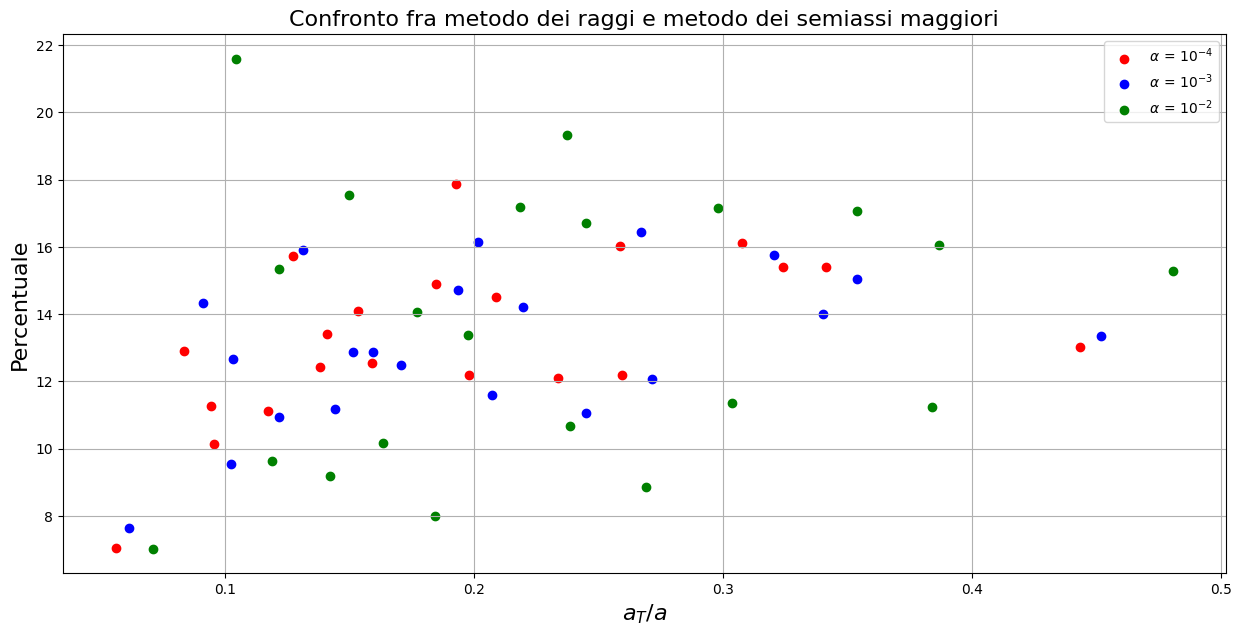
\includegraphics[width=\textwidth]{Immagini/Risultati/discr_disc.png}
  \caption{Confronto fra il metodo dei raggi ed il metodo dei semiassi per la determinazione delle dimensioni del disco. Notiamo come le variazioni non abbiano una dipendenza evidente sulla viscosità $\alpha$ e oscillino fra il $10\%$ ed il $20\%$.}
  \label{fig:discr_disc}
\end{figure}

\section{Eccentricità del disco} \label{sec:ecc_disc}

Abbiamo definito $e_{disco}$ come il valore medio dell'eccentricità delle orbite nell'intorno del semiasse di troncamento (vedi Sezione \ref{sec:metnum_anal}). Come per le dimensioni del disco, le stime d'eccentricità che forniamo per i sistemi analizzati sono le medie temporali effettuate fra la trentesima e la cinquantesima orbita del sistema binario.
In Figura \ref{fig:edisco_alfa2}, \ref{fig:edisco_alfa3} ed \ref{fig:edisco:alfa4} sono riportati i risultati delle analisi che abbiamo effettuato: i valori numerici possono essere consultati in Appendice \ref{appendiceE}.
I grafici con cui presentiamo i risultati sono analoghi a quelli utilizzati in precedenza per le dimensioni dei dischi: sulle ascisse è posto il rapporto $m_{cen}/m_{per}$, dove $m_{cen}$ indica la massa della stella posta al centro della griglia, mentre $m_{per}$ quella del corpo perturbante. Sulle ordinate si trova l'eccentricità $e$ della binaria. 
Il colore delle celle è dettato dal valore di $e_{disco}$ dell'oggetto in analisi: gli estremi della scala sono la massima e la minima eccentricità ottenuta.

Abbiamo osservato che tutti i valori numerici appartengono all'intervallo $e_{disco}\,\in\,[0.05,\,0.42]$.
Le maggiori $e_{disco}$ sono quelle dei dischi circum-secondari: supponiamo che la spiegazione di questo fenomeno siano le forze mareali più intense causate dal corpo principale della binaria.

Notiamo che l'eccentricità dei dischi diminuisce in media all'aumentare di $e$: il maggior troncamento che subiscono i dischi in un sistema binario altamente eccentrico fa si che non sia presente materiale in corrispondenza delle risonanze che eccitano $e_{disco}$. Il risultato è la presenza di strutture orbitanti più circolari.

\begin{figure}[H]
  \centering
  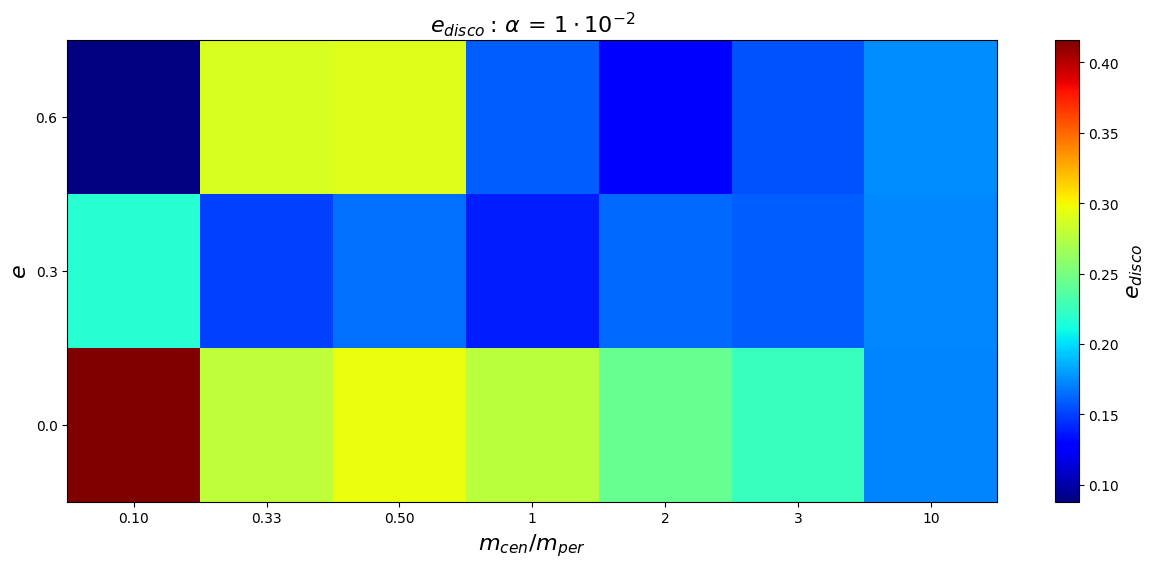
\includegraphics[width=\textwidth]{Immagini/Risultati/edisco_alfa2.png}
  \caption{Valori di $e_{disco}$ per $\alpha\,=\,1\cdot 10^{-2}$}
  \label{fig:edisco_alfa2}
\end{figure}

\begin{figure}[H]
  \centering
  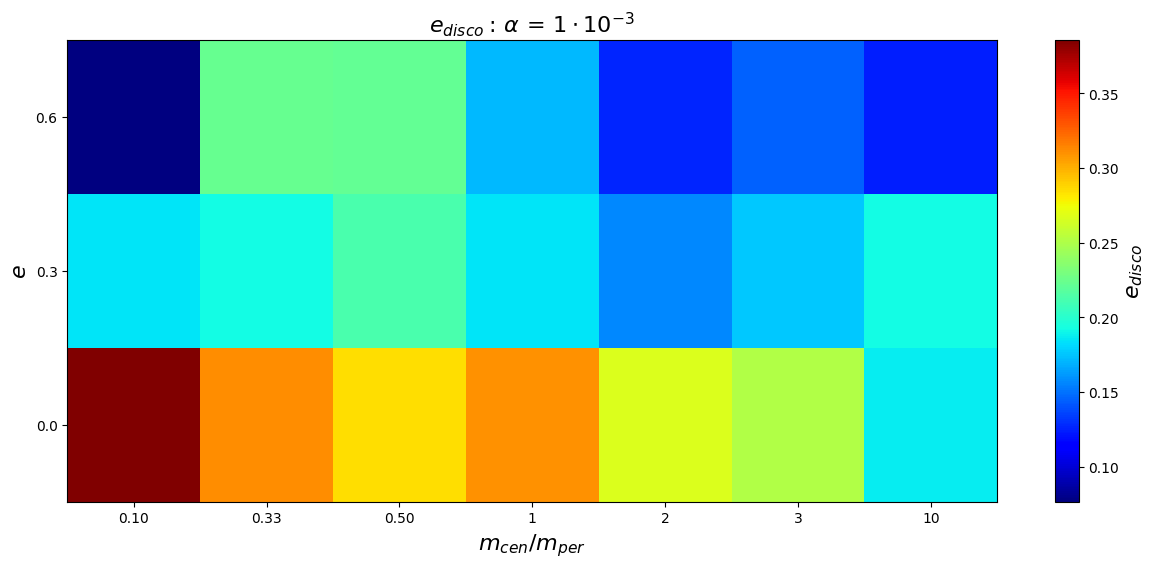
\includegraphics[width=\textwidth]{Immagini/Risultati/edisco_alfa3.png}
  \caption{Valori di $e_{disco}$ per $\alpha\,=\,1\cdot 10^{-3}$}
  \label{fig:edisco_alfa3}
\end{figure}

\begin{figure}[H]
  \centering
  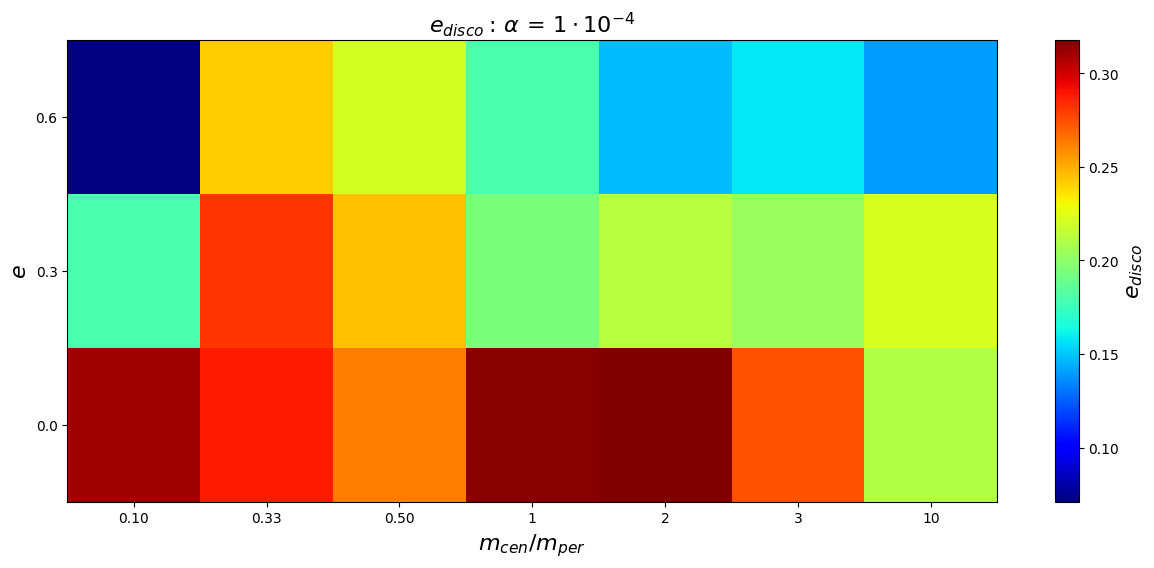
\includegraphics[width=\textwidth]{Immagini/Risultati/edisco_alfa4.png}
  \caption{Valori di $e_{disco}$ per $\alpha\,=\,1\cdot 10^{-4}$}
  \label{fig:edisco:alfa4}
\end{figure}

In Figura \ref{fig:riass_edisco} è resa più evidente la dipendenza dall'eccentricità della binaria. Sulle ascisse del grafico è posta la dimensione del disco $a_T/a$, mentre le ordinate ospitano i valori di $e_{disco}$.
I punti costituenti il grafico a dispersione sono colorati in base all'eccentricità del sistema binario al quale appartengono: è evidente come i massimi valori di $e_{disco}$ siano ottenuti per $e\,=\,0.0$

\begin{figure}[h]
  \centering
  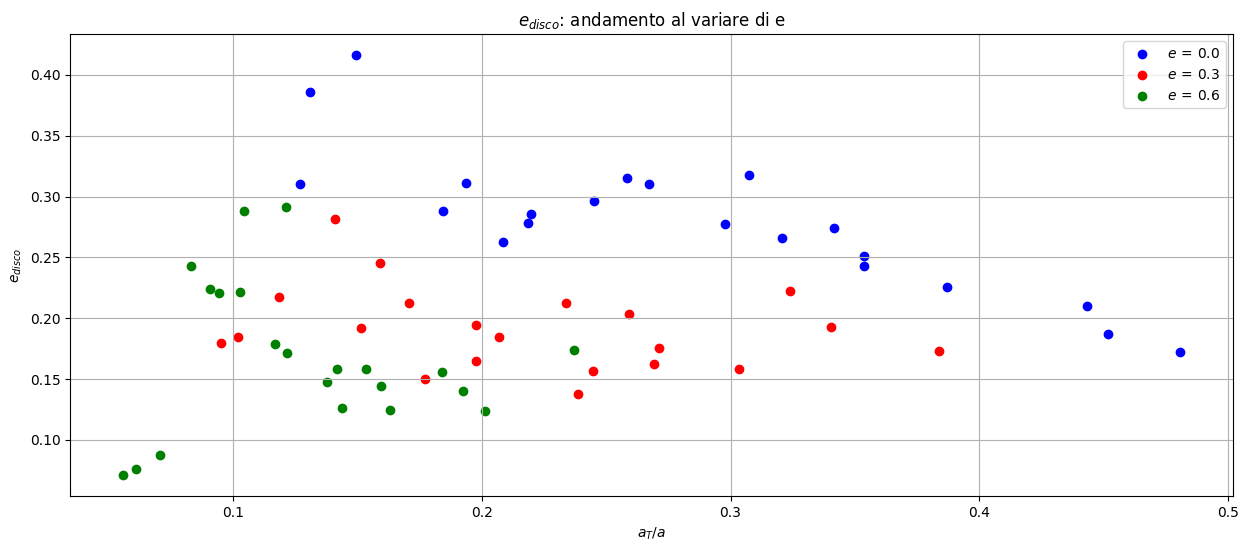
\includegraphics[width=\textwidth]{Immagini/Risultati/riassuntivo_edisco.png}
  \caption{Grafico riassuntivo delle stime di $e_{disco}$ effettuate: è evidente una dipendenza sull'eccentricità del sistema binario considerato. Oltre a diminuire in dimensione, i dischi in analisi presentano eccentricità inferiori all'aumentare di $e$.}
  \label{fig:riass_edisco}
\end{figure}


\section{Confronto con i risultati teorici} \label{sec:conf_teo}

In questa sezione effettuiamo il confronto con le predizioni teoriche del modello di \textcite{ManaraTronc2019}. 
La formula \eqref{eq:tronc_disc} presenta quattro parametri: i primi due, ossia $a$ e $b$, hanno una dipendenza sulla viscosità del materiale costituente il disco.
In questo lavoro di tesi abbiamo lavorato con tre diversi parametri adimensionali $\alpha\,\in \{10^{-2},\,10^{-3},\,10^{-4}\}$.
\'E possibile valutare i corrispondenti numeri di Reynolds secondo
\begin{equation}
R\,=\,\frac{1}{\alpha} \left(\frac{h}{r}\right)^{-2},
\label{eq:rey_disc}
\end{equation}
dove in $h/r$ riconosciamo l'aspect-ratio del disco. I corrispettivi $R$ sono: $4 \cdot 10^4$, $4 \cdot 10^5$, $4 \cdot 10^6$.
I valori di $a$, $b$ sono stati forniti da \textcite{ManaraTronc2019} (vedi Appendice \ref{appendiceA}) per $R\,=\,10^4,\,10^5,\,10^6$: per effettuare un confronto più corretto abbiamo estrapolato linearmente i parametri per $R\,=\,4\cdot 10^4,\,4\cdot10^5$.
L'estrapolazione fornisce risultati errati per $R\,=\,4 \cdot 10^6$ poiché è un numero di Reynolds esterno al range campionato: per tali dati utilizziamo come $a$, $b$ di riferimento quelli proposti da \textcite{ManaraTronc2019} nel caso di $R\,=\,10^6$. I valori ottenuti in questa fase dell'analisi sono riportati in Tabella \ref{tab:para_conf_estr1}.

A viscosità del materiale fissata $a$, $b$ dipendono dalla massa ridotta $\mu\,=\,m_2/(m_1+m_2)$: dato che i valori da noi utilizzati non corrispondono con quelli riportati nel paper di \textcite{ManaraTronc2019}, effettuiamo una seconda estrapolazione su $\mu$.
I parametri definitivi $a$, $b$ che abbiamo utilizzato per effettuare i confronti sono riportati in Tabella \ref{tab:para_conf_estr2}.\\

La relazione \eqref{eq:tronc_disc} consente di determinare le dimensioni del raggio di troncamento: abbiamo deciso di effettuare il confronto sia per i valori di $r_T$ che abbiamo individuato, che per quelli di $a_T$. 
Il motivo per cui abbiamo deciso di confrontare gli $a_T$ da noi determinati con i risultati forniti dalla relazione individuata da \textcite{ManaraTronc2019} è che vogliamo investigare se il formalismo dei semiassi maggiori fornisca dei riscalamenti al variare di $m_2/m_1$ analoghi a quelli dei raggi di troncamento.\\

I grafici con cui presentiamo il confronto con la legge analitica per la determinazione di $r_T$ sono tutti dello stesso tipo: sulle ascisse abbiamo posto la coordinata radiale riscalata in unità del semiasse maggiore della binaria, mentre sulle ordinate si trova il rapporto $m_2/m_1$ fra le masse della stella secondaria e di quella principale.
Le predizioni teoriche sono riportate in colore nero, la regione colorata di azzurro e delimitata da delle linee blu è quella occupata dal disco circum-primario, mentre il colore rosso definisce l'estensione spaziale del disco circum-secondario.

\subsection{Raggi di troncamento}

Abbiamo definito $r_T$ come il raggio del cerchio centrato nell'origine della griglia di simulazione contente il $99.9\%$ della massa presente nella regione considerata. 
Il criterio che abbiamo fornito è differente da quello di \textcite{ArtymowiczLubow1994}, che consideravano il disco troncato nella posizione spaziale dove la densità del materiale orbitante era metà di quella massima.
Notiamo che le estensioni spaziali dei dischi da noi ottenute risultano in media maggiori rispetto a quelle aspettate secondo la relazione suggerita da \textcite{ManaraTronc2019}.\\

\textbf{Viscosità massima}\\

Il caso di viscosità massima è quello che corrisponde ad $\alpha\,=\,10^{-2}$. 
Nel caso di binaria circolare notiamo un buon accordo fra le predizioni teoriche ed i risultati numerici: le discrepanze con il modello sono minime.
Per le simulazioni effettuate con $e\,=\,0.3$ osserviamo che i $r_T$ da noi ottenuti sono maggiori rispetto a quelli di \textcite{ManaraTronc2019}: il disco circum-primario teorico con $m_2/m_1\,=\,0.1$ risulta il $13\%$ più piccolo rispetto a quanto da noi ottenuto.
Le discrepanze con il modello risultano maggiori per il circum-primario a bassi $m_2/m_1$, mentre accade il contrario per il circum-secondario.
Nel caso di binaria altamente eccentrica $e\,=\,0.6$ le predizioni della \eqref{eq:tronc_disc} risultano essere maggiormente compatibili con le simulazioni effettuate: la massima discrepanza si verifica per il disco circum-secondario con $m_2/m_1\,=\,0.5$ ed è pari all' $8\%$ di $r_T$.
\begin{figure}[H]
  \centering
  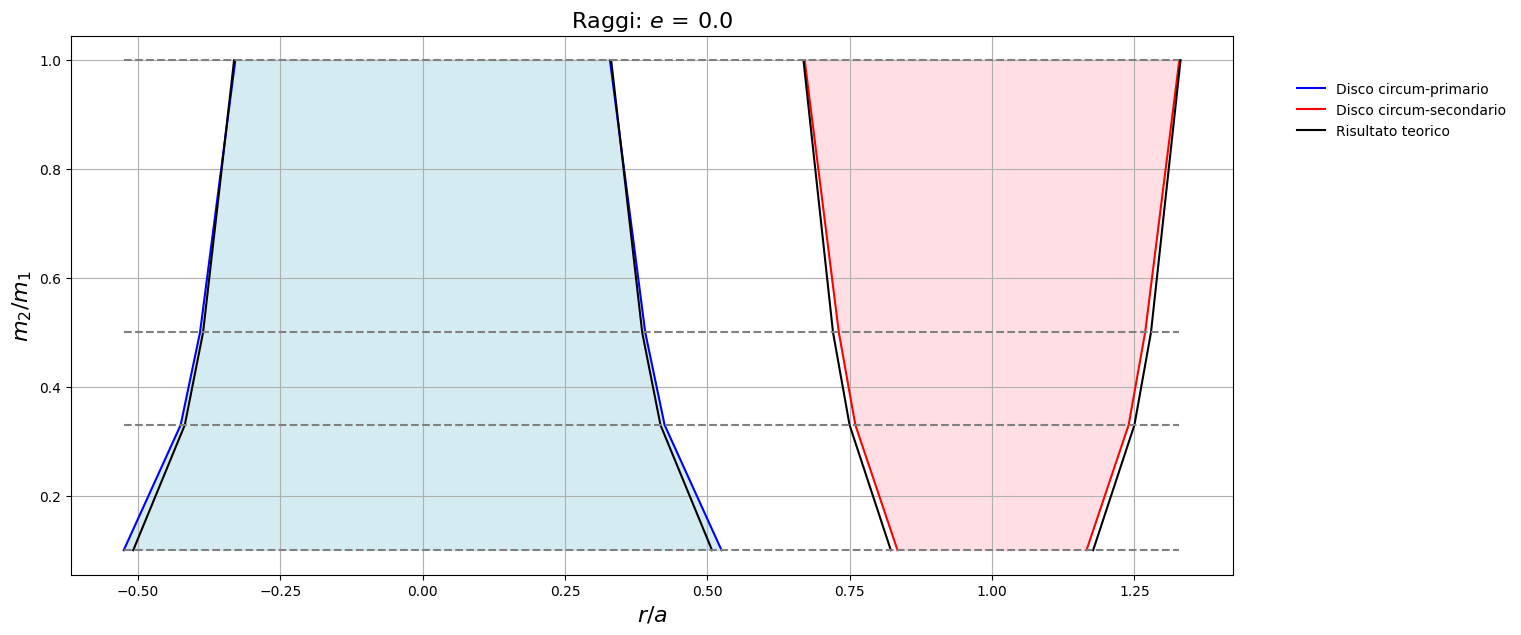
\includegraphics[width=\textwidth]{Immagini/Confronto/conrag_A2_e0.png}
  \caption{Confronto fra predizioni teoriche del raggio di troncamento e valori numerici di $r_T$. I dischi considerati in questo grafico hanno $\alpha\,=\,1 \cdot 10^{-2}$ e sono ospitati in un sistema binario con eccentricità $e\,=\,0.0$. }
  \label{fig:conf_rag20}
\end{figure}

\begin{figure}[H]
  \centering
  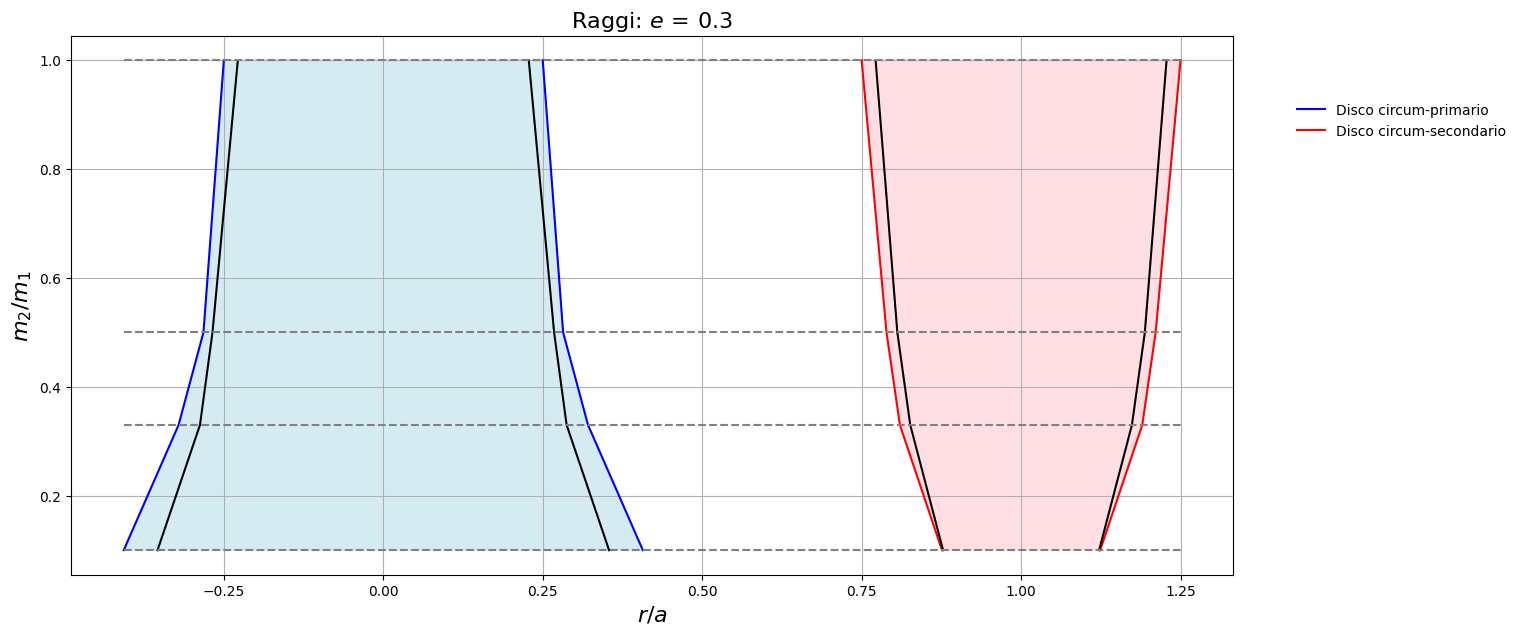
\includegraphics[width=\textwidth]{Immagini/Confronto/conrag_A2_e3.png}
  \caption{Differenze fra i risultati teorici ed i valori numeri del raggio di troncamento. I dischi riportati in figura sono costituiti da materiale con viscosità $\alpha\,=\,10^{-2}$: l'eccentricità del sistema binario è $e\,=\,0.3$. Notiamo come i dischi da noi ottenuti risultino più estesi di quelli predetti dalla $\eqref{eq:tronc_disc}$: l'andamento per piccoli $m_2/m_1$ da noi individuato differisce da quello individuato da \textcite{ManaraTronc2019}.}
  \label{fig:conf_rag23}
\end{figure}

\begin{figure}[H]
  \centering
  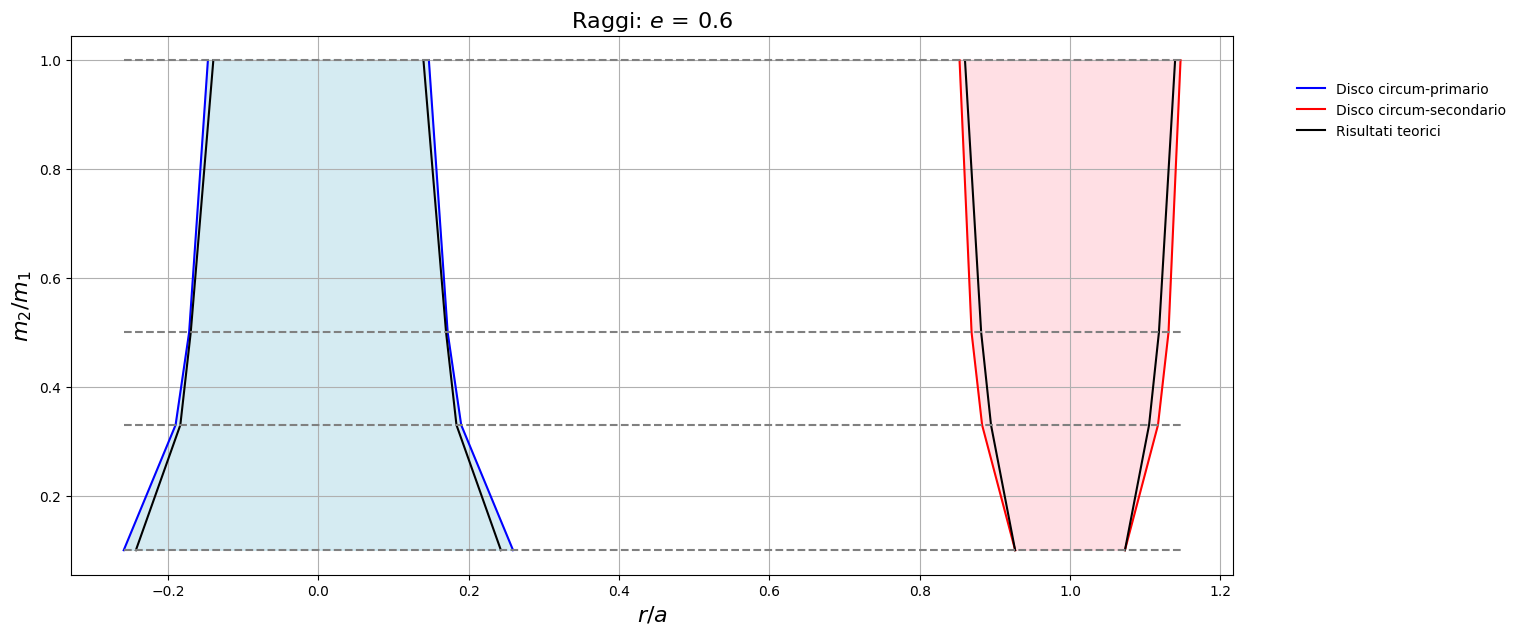
\includegraphics[width=\textwidth]{Immagini/Confronto/conrag_A2_e6.png}
  \caption{Confronto fra il modello di \textcite{ManaraTronc2019} e i risultati numerici per del materiale caratterizzato da $\alpha\,=\,10^{-2}$ orbitante in un sistema ad elevata eccentricità. Gli andamenti sono confrontabili: la discrepanza maggiore, pari all' $8\%$ di $r_T$, si presenta per il disco circum-secondario della binaria con $m_2/m_1\,=\,0.5$.}
  \label{fig:conf_rag26}
\end{figure}

\newpage
\textbf{Viscosità media}\\

I dischi a viscosità media sono caratterizzati da $\alpha\,=\,10^{-3}$, che corrisponde ad un numero di Reynolds pari a $R\,=\,4 \cdot 10^5$.
Come per $\alpha\,=\,10^{-2}$, i raggi di troncamento ottenuti mediante simulazione risultano maggiormente in disaccordo con il modello teorico quando $e\,=\,0.3$.

Nel caso di binaria circolare è presente un buon accordo fra i valori numerici e quelli ottenuti mediante la \eqref{eq:tronc_disc}: osserviamo che il disco circum-secondario per ogni valore del rapporto $m_2/m_1$ risulta più piccolo della predizione teorica, sebbene venga descritta correttamente la dipendenza da $q$ (vedi Figura \ref{fig:conf_rag30}).
Per i dischi appartenenti al sistema binario mediamente eccentrico osserviamo che le dimensioni del disco circum-primario risultano superiori a quelle ottenute con la relazione di \textcite{ManaraTronc2019}: in termini percentuali la differenza fra $r_T$ simulati e teorici raggiunge il $21\%$ (vedi Figura \ref{fig:conf_rag33}).
Nel caso di binaria con $e\,=\,0.6$ i valori numerici risultano maggiori rispetto a quelli ottenuti con la \eqref{eq:tronc_disc}: osserviamo che la dipendenza dal rapporto $m_2/m_1$ è la stessa dei risultati presenti in letteratura (vedi Figura \ref{fig:conf_rag36}).


\begin{figure}[H]
  \centering
  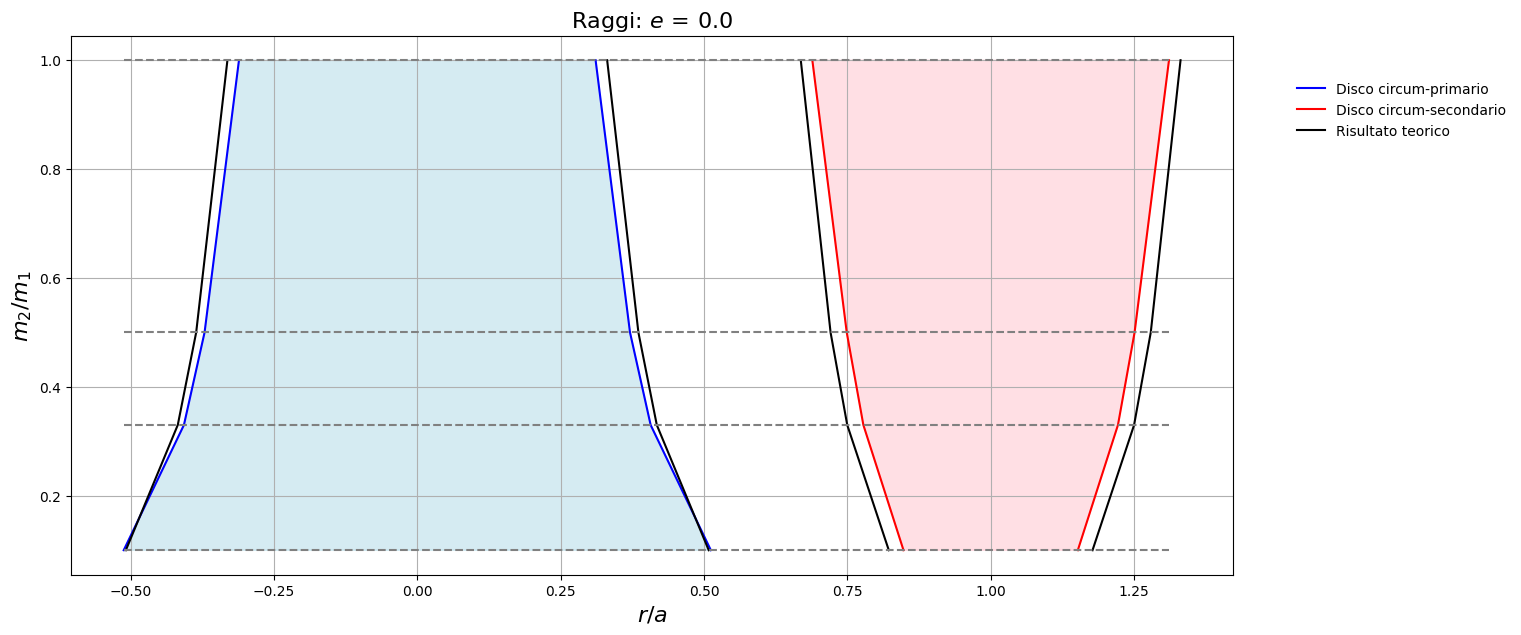
\includegraphics[width=\textwidth]{Immagini/Confronto/conrag_A3_e0.png}
  \caption{Confronto fra risultati numerici ed i valori teorici per dischi costituiti da materiale con $\alpha\,=\,10^{-3}$ appartenenti ad un sistema binario circolare. Le dimensioni dei dischi circum-secondari ottenute per via simulativa risultano essere inferiori rispetto a quelle suggerite dalla \eqref{eq:tronc_disc}: notiamo che l'andamento in dipendenza del rapporto $m_2/m_1$ è lo stesso per le due tipologie di stima di $r_T$. Il disco circum-primario è coerente con la relazione proposta da \textcite{ManaraTronc2019} per piccoli $q$, mentre per grandi valori risulta leggermente più piccolo.}
  \label{fig:conf_rag30}
\end{figure}

\begin{figure}[H]
  \centering
  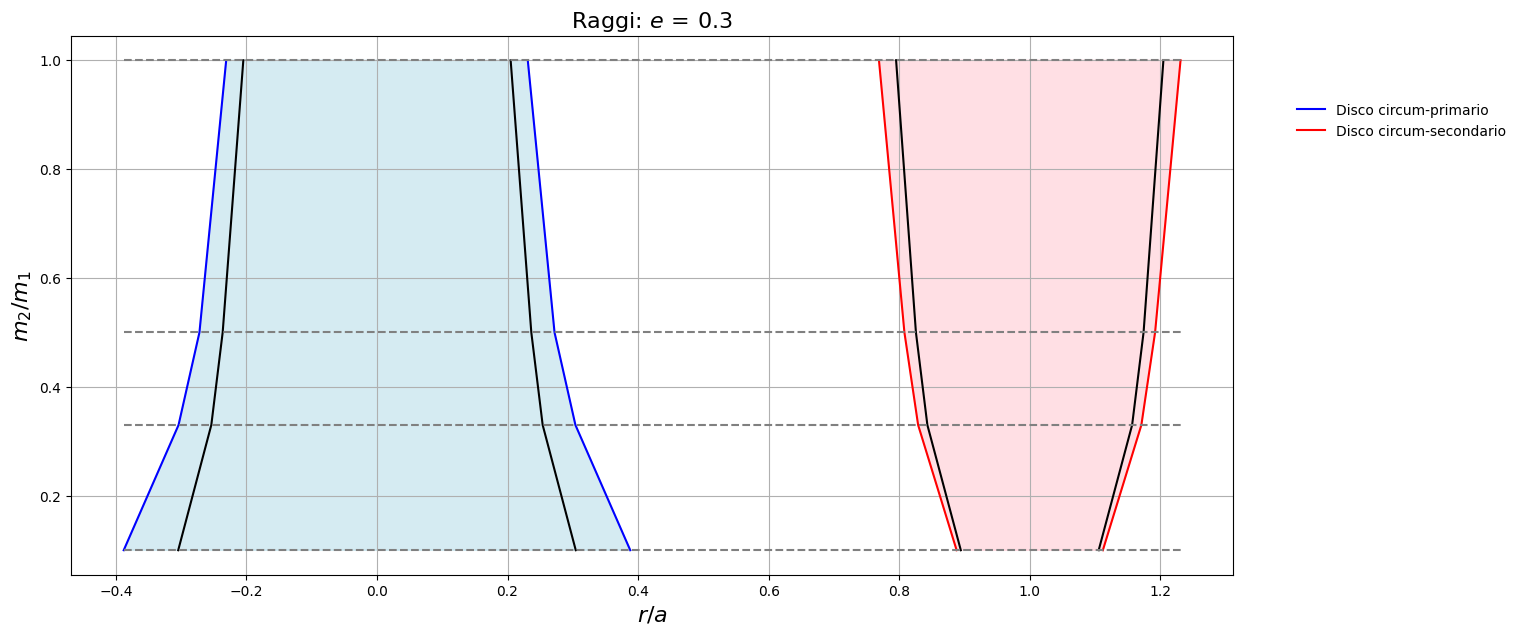
\includegraphics[width=\textwidth]{Immagini/Confronto/conrag_A3_e3.png}
  \caption{Paragone fra le dimensioni ottenute numericamente e quelle determinate mediante la relazione proposta da \textcite{ManaraTronc2019} per dischi caratterizzati da  $\alpha\,=\,10^{-3}$ ospitati in un sistema binario mediamente eccentrico Notiamo che il disco circum-primario presenta una dipendenza da $m_2/m_1$ è differente, poiché per bassi valori di $q$ tende ad allargarsi maggiormente. Il disco circum-secondario presenta un buon accordo con la \eqref{eq:tronc_disc} per piccoli $q$, mentre tende ad espandersi più di quanto predetto dal modello per alti valori di $m_2/m_1$.}
  \label{fig:conf_rag33}
\end{figure}

\begin{figure}[H]
  \centering
  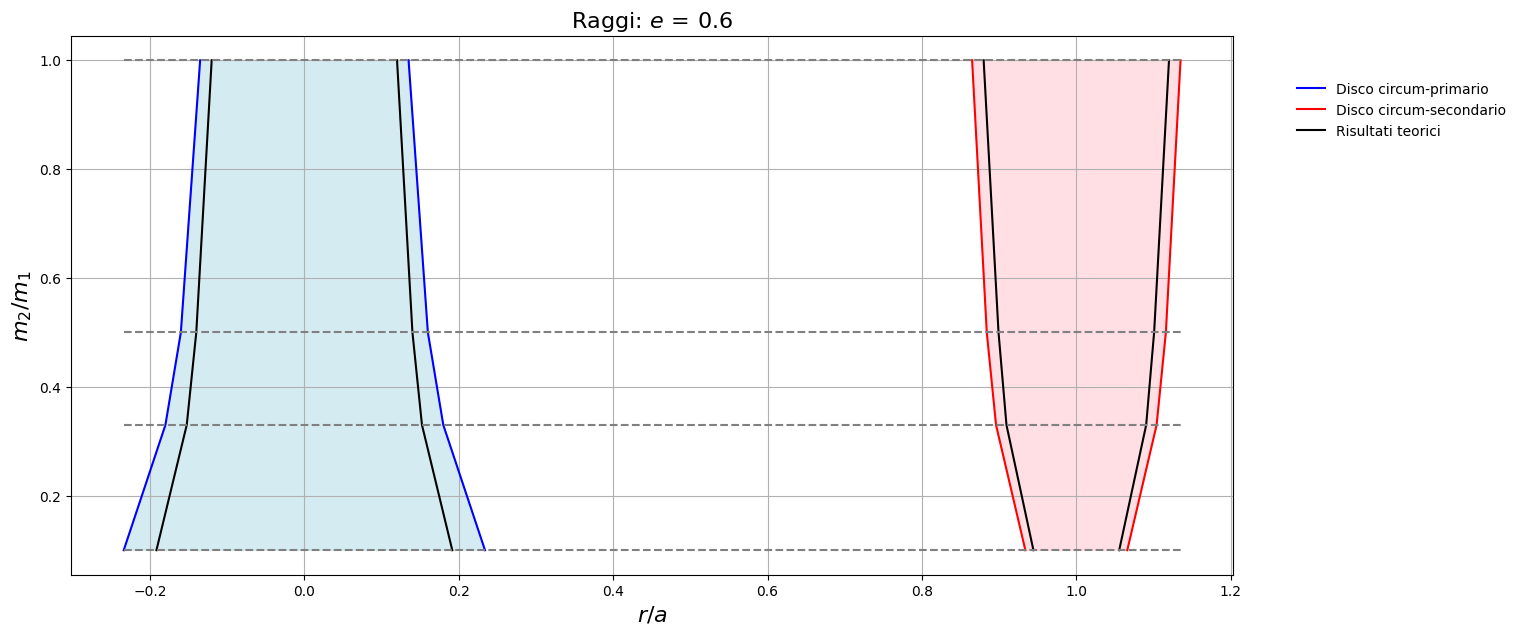
\includegraphics[width=\textwidth]{Immagini/Confronto/conrag_A3_e6.png}
  \caption{In figura sono riportate le regioni occupate dai dischi circumstellari al variare del mass-ratio del sistema altamente eccentrico del quale fanno parte: il materiale costituente i dischi ha $\alpha\,=\,10^{-3}$. Gli andamenti numerici che abbiamo ottenuto sono paragonabili a quelli teorici determinati secondo la relazione \eqref{eq:tronc_disc}: le dimensioni di entrambi i dischi risultano tuttavia maggiori di quanto proposto dal modello a cui stiamo facendo riferimento. }
  \label{fig:conf_rag36}
\end{figure}

\textbf{Viscosità minima}\\

I dischi a viscosità minima sono quelli costituiti da materiale caratterizzato da $\alpha\,=\,10^{-4}$: il corrispondente numero di Reynolds è $R\,=\,4 \cdot 10^{6}$. 
I confronti con il modello teorico per le dimensioni di tali oggetti sono le meno significative presenti in questo lavoro di tesi: i paragoni che ci apprestiamo ad analizzare sono effettuati con l'andamento teorico previsto per $R\,=\,1 \cdot 10^{6}$, poiché il numero di Reynolds a cui stiamo lavorando si trova al di fuori dell'intervallo investigato da \textcite{ManaraTronc2019}.

Come nel caso precedente, notiamo che entrambi i dischi facenti parte di una binaria circolare risultano essere leggermente più piccoli di quanto predetto dalla \eqref{eq:tronc_disc} (vedi Figura \ref{fig:conf_rag40}). In particolare il disco circum-secondario risulta meno esteso del modello teorico per ogni $m_2/m_1$ campionato: la massima differenza percentuale si verifica per $m_2/m_1\,=\,0.33$ ed è del $18\%$.
La binaria mediamente eccentrica $e\,=\,0.3$ si verifica nuovamente la casistica con maggior differenze fra le predizioni della \eqref{eq:tronc_disc} ed i valori da noi determinati: il disco circum-primario presenta un incremento in dimensioni maggiore rispetto al modello teorico per piccoli $m_2/m_1$ (vedi Figura \ref{fig:conf_rag43}).
Entrambi i dischi circumstellari con $e\,=\,0.6$ risultano più grandi delle predizioni di \textcite{ManaraTronc2019}: la massima differenza percentuale è del $26\%$ per il disco circum-primario a $m_2/m_1\,=\,0.1$ (vedi Figura \ref{fig:conf_rag46}). 

\begin{figure}[H]
  \centering
  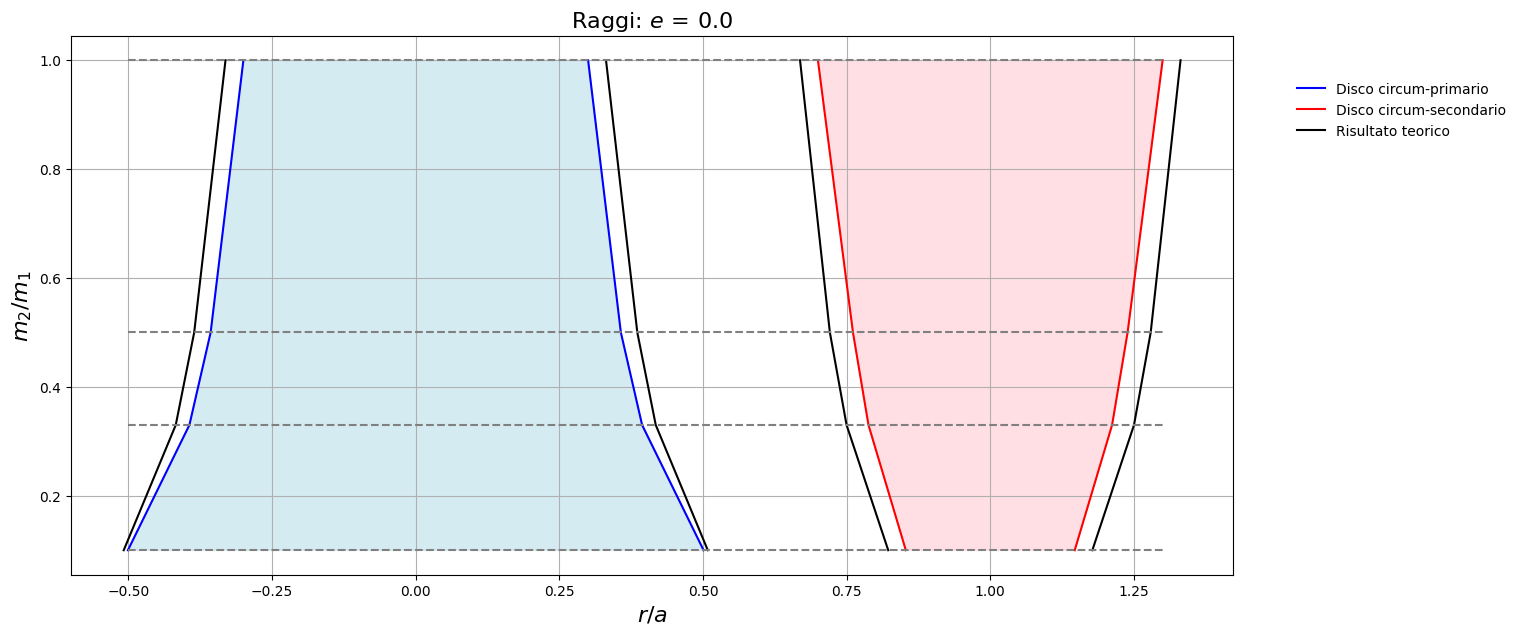
\includegraphics[width=\textwidth]{Immagini/Confronto/conrag_A4_e0.png}
  \caption{In Figura è riportato il confronto fra i valori numerici e le predizioni teoriche della relazione proposta da \textcite{ManaraTronc2019} per dei dischi caratterizzati da $\alpha\,=\,10^{-4}$ orbitanti in una binaria circolare. Osserviamo come il disco circum-secondario presenta dei raggi di troncamento più piccoli rispetto alle predizioni teoriche per ogni valore di $m_2/m_1$.}
  \label{fig:conf_rag40}
\end{figure}

\begin{figure}[H]
  \centering
  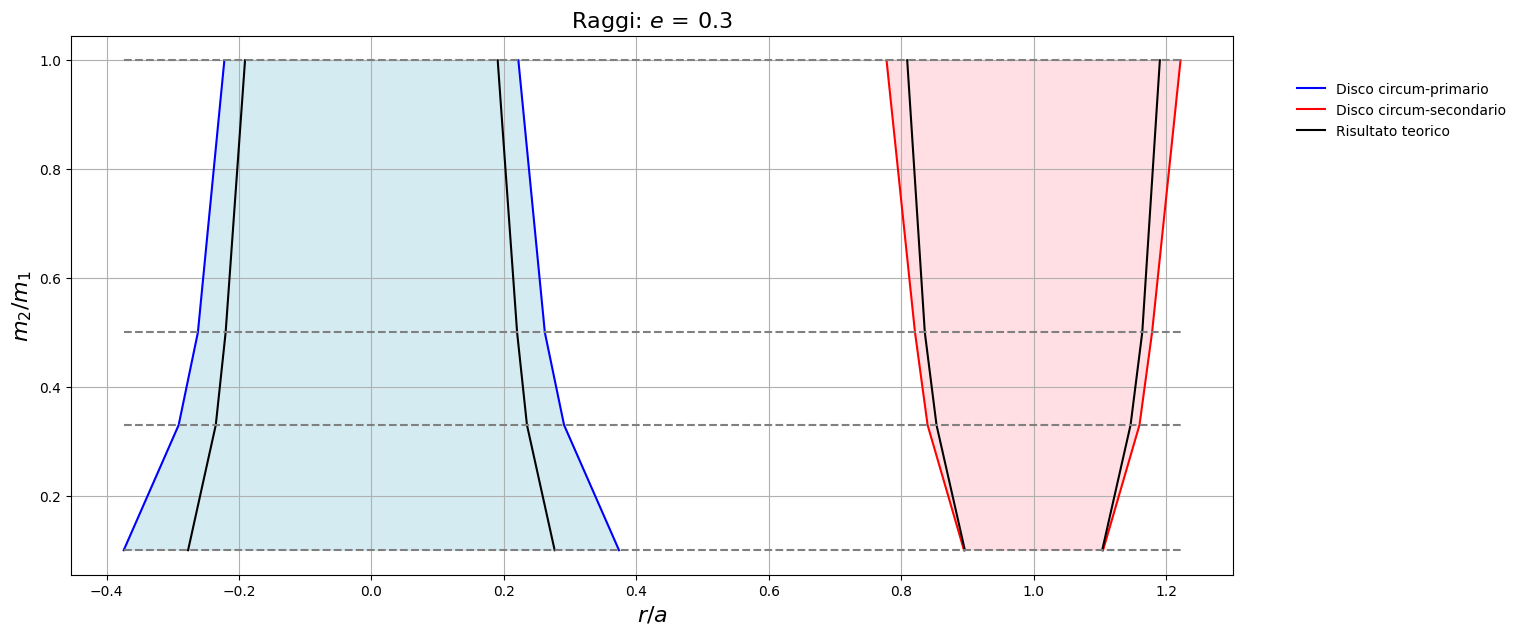
\includegraphics[width=\textwidth]{Immagini/Confronto/conrag_A4_e3.png}
  \caption{Paragone fra le simulazioni da noi effettuate e le predizioni teoriche per le dimensioni di dischi circumstellari costituiti da materiale con $\alpha\,=\,10^{-4}$ ospitati in un sistema binario a media eccentricità. Il disco circum-primario numericamente ottenuto é maggiormente esteso rispetto alle predizioni teoriche per ogni valore del rapporto $m_2/m_1$: la massima differenza è presente per bassi valori di $q$. Il disco circum-secondario presenta un comportamento opposto, in quanto per alti $m_2/m_1$ risulta più grande di quanto suggerito dalla teoria.}
  \label{fig:conf_rag43}
\end{figure}

\begin{figure}[H]
  \centering
  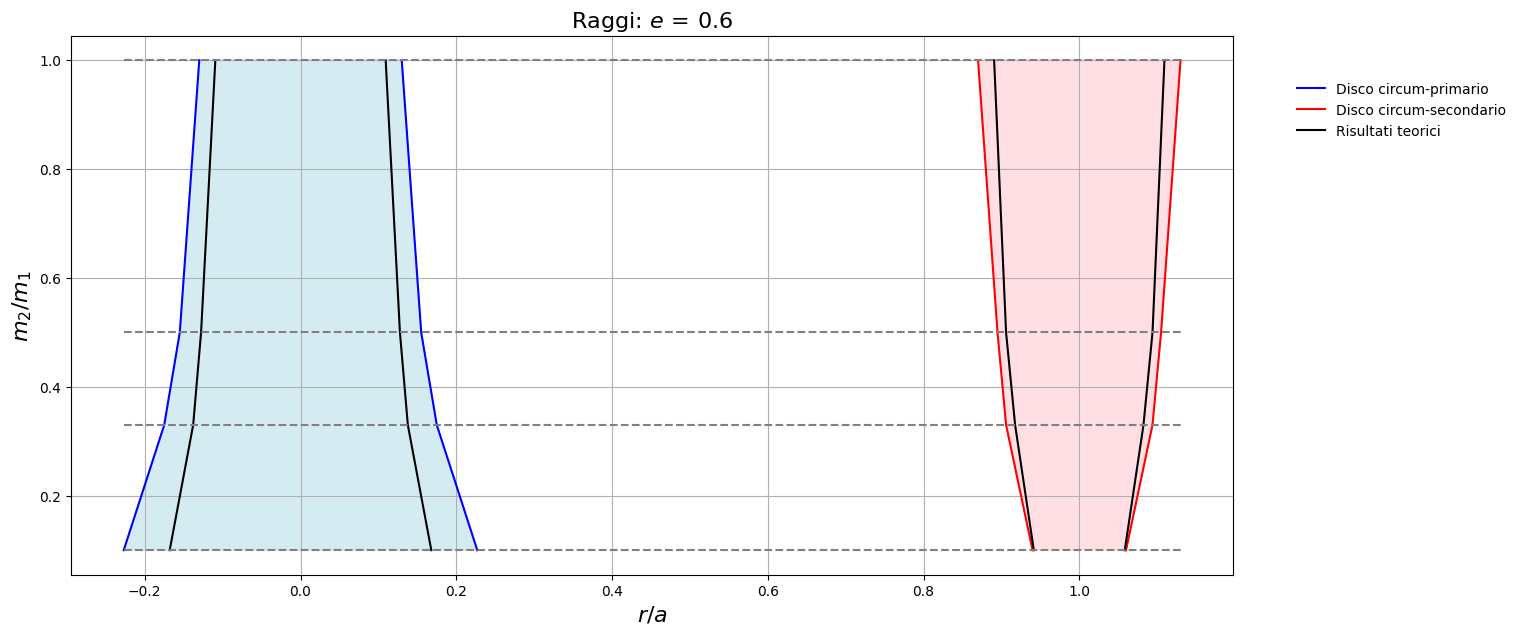
\includegraphics[width=\textwidth]{Immagini/Confronto/conrag_A4_e6.png}
  \caption{In figura sono riportate le regioni occupate da dei dischi circumstellari con $\alpha\,=\,10^{-4}$ in un sistema altamente eccentrico al variare di $m_2/m_1$. Osserviamo che sia il disco circum-primario, che quello circum-secondario risultano di dimensioni maggiori rispetto al modello teorico. La massima differenza è presente per il materiale orbitante attorno alla componente principale della binaria per $m_2/m_1\,=\,0.1$}
  \label{fig:conf_rag46}
\end{figure}

\subsection{Semiassi di troncamento}

Abbiamo definito come $a_T$ il semiasse maggiore  dell'orbita del materiale tale che il $99.9\%$ del materiale presente nella griglia simulativa compisse orbite a semiassi inferiori.
Lavorando in termini di $a_T$ dovremmo essere in grado di evitare una problematica riportata da \textcite{ArtymowiczLubow1994}, ossia che la determinazione delle dimensioni del disco d'accrescimento è resa difficoltosa dalla sua mancanza di simmetria per rotazione attorno all'asse z.

Abbiamo osservato, come riportato nella Sottosezione \ref{subsec:semiax_tr}, che le dimensioni dei dischi ricavate con il metodo dei semiassi maggiori sono inferiori rispetto a quelle dei raggi di troncamento.
Di conseguenza, il confronto con il modello proposto da \textcite{ManaraTronc2019} fornisce dei risultati differenti.
I dischi ospitati in binarie circolari sono più piccoli rispetto alle predizioni teoriche, sebbene il modo di scalare al variare di $m_2/m_1$ sia lo stesso per i valori simulati e quelli ottenuti con la \eqref{eq:tronc_disc}.
Per i dischi facenti parte di sistemi binari a media o alta eccentricità l'accordo con il modello teorico è molto elevato.
Abbiamo osservato per tutti i valori di $\alpha$ che l'andamento proposto da \textcite{ManaraTronc2019} al variare di $m_2/m_1$ è altamente compatibile con quello ottenuto per il metodo dei semiassi.\\

\textbf{Viscosità massima}\\

Il materiale a viscosità massima è caratterizzato da $\alpha\,=\,10^{-2}$. 
Osserviamo che nelle binarie circolari sia il disco circum-primario che quello circum-secondario sono di taglia inferiore rispetto alle predizioni teoriche (vedi Figura \ref{fig:conf_ax20}).

\begin{figure}[H]
  \centering
  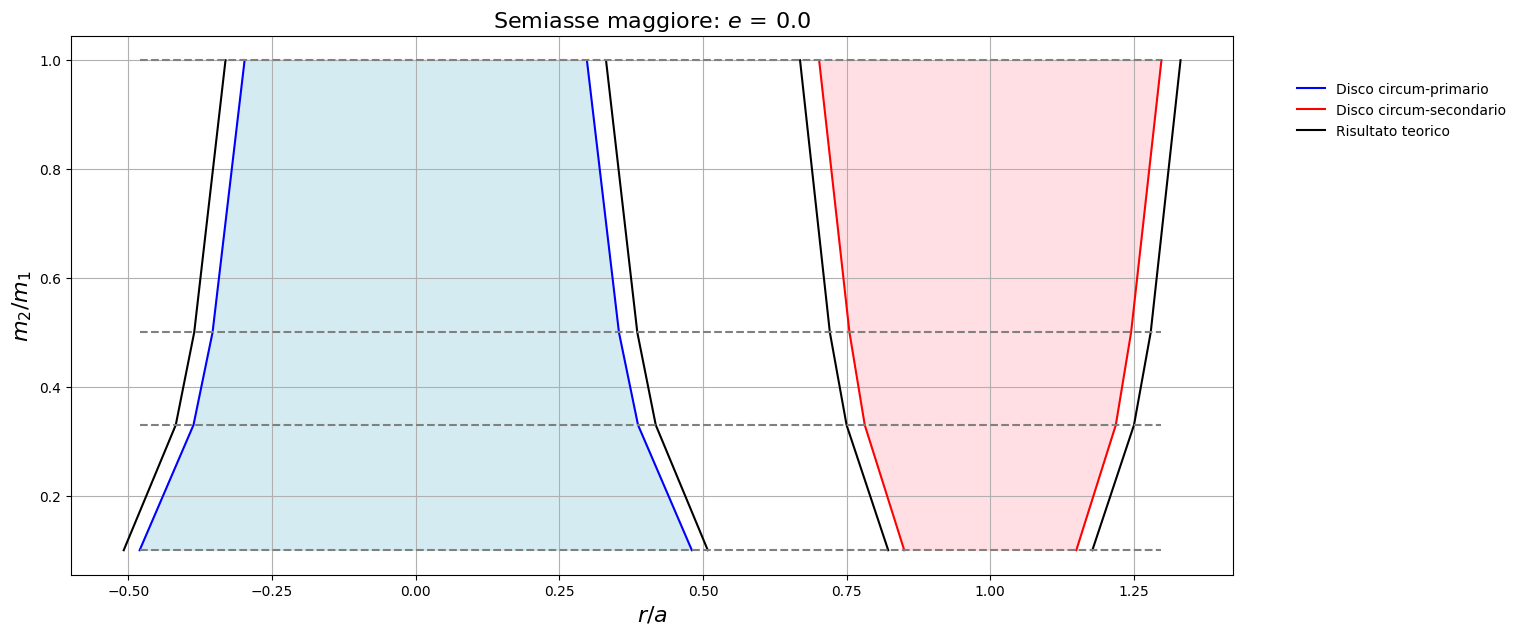
\includegraphics[width=\textwidth]{Immagini/Confronto/confax_A2_e0.png}
  \caption{Confronto fra modello e valori numerici per $\alpha\,=\,10^{-2}$ per dischi ospitati in un sistema binario circolare. Osserviamo che sia entrambi i tipi di dischi da noi ottenuti sono di dimensioni inferiori alle predizioni della \ref{eq:tronc_disc}}
  \label{fig:conf_ax20}
\end{figure}

I dischi in sistemi ad $e\,=\,0.3$ ed $e\,=\,0.6$ presentano un elevato accordo con le predizioni teoriche (vedi Figure \ref{fig:conf_ax23}, \ref{fig:conf_ax26}).

\begin{figure}[H]
  \centering
  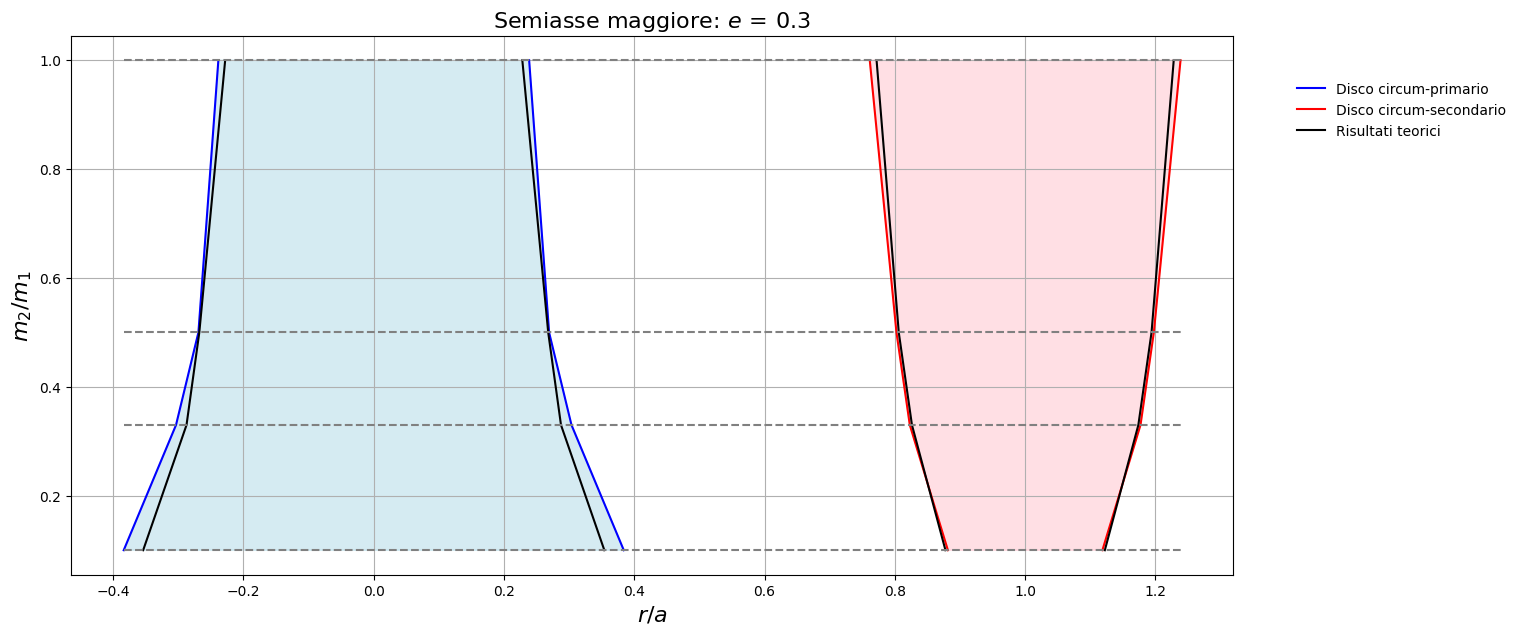
\includegraphics[width=\textwidth]{Immagini/Confronto/confax_A2_e3.png}
  \caption{Confronto fra predizioni teoriche di $r_T$ e dimensioni dei dischi con il metodo dei semiassi per $\alpha\,=\,10^{-2}$ ed $e\,=\,0.3$. Osserviamo un elevata compatibilià fra modello e valori numerici, sebbene la dipendenza su $m_2/m_1$ da noi individuata per il disco circum-primario risulta essere leggermente differente, con maggiori espansioni a bassi ed alti $q$.}
  \label{fig:conf_ax23}
\end{figure}

\begin{figure}[H]
  \centering
  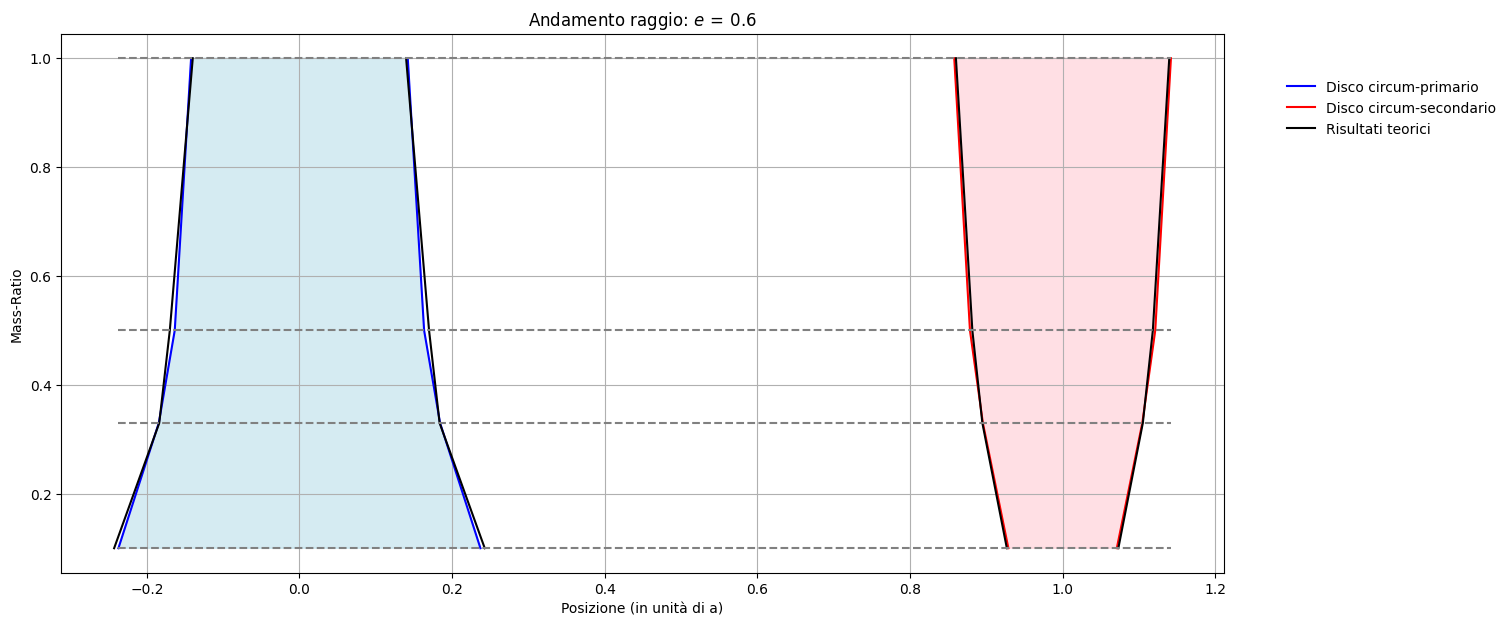
\includegraphics[width=\textwidth]{Immagini/Confronto/confax_A2_e6.png}
  \caption{In figura è riportato un paragone fra il modello di \textcite{ManaraTronc2019} e i valori numerici da noi calcolati. I dischi in questione hanno $\alpha\,=\,10^{-2}$ ed $e\,=\,0.6$: osserviamo come le due stime risultino coincidenti, con andamenti al variare di $m_2/m_1$ totalmente sovrapponibili.}
  \label{fig:conf_ax26}
\end{figure}

\textbf{Viscosità media}\\

I dischi a viscosità media sono costituiti da materiale caratterizzato da $\alpha\,=\,10^{-3}$. 
Osserviamo che nel caso di binaria circolare entrambi i dischi presentano delle dimensioni inferiori a quelle del modello teorico, sebbene il modo di scalare al variare di $m_2/m_1$ sia confrontabile (vedi Figura \ref{fig:conf_ax30}).
I dischi circum-primari con $e\,=\,0.3$ risultano più estesi delle predizioni teoriche per bassi $m_2/m_1$, mentre i circum-secondari sono in perfetto accordo con la \ref{eq:tronc_disc} (vedi Figura \ref{fig:conf_ax33}).

\begin{figure}[H]
  \centering
  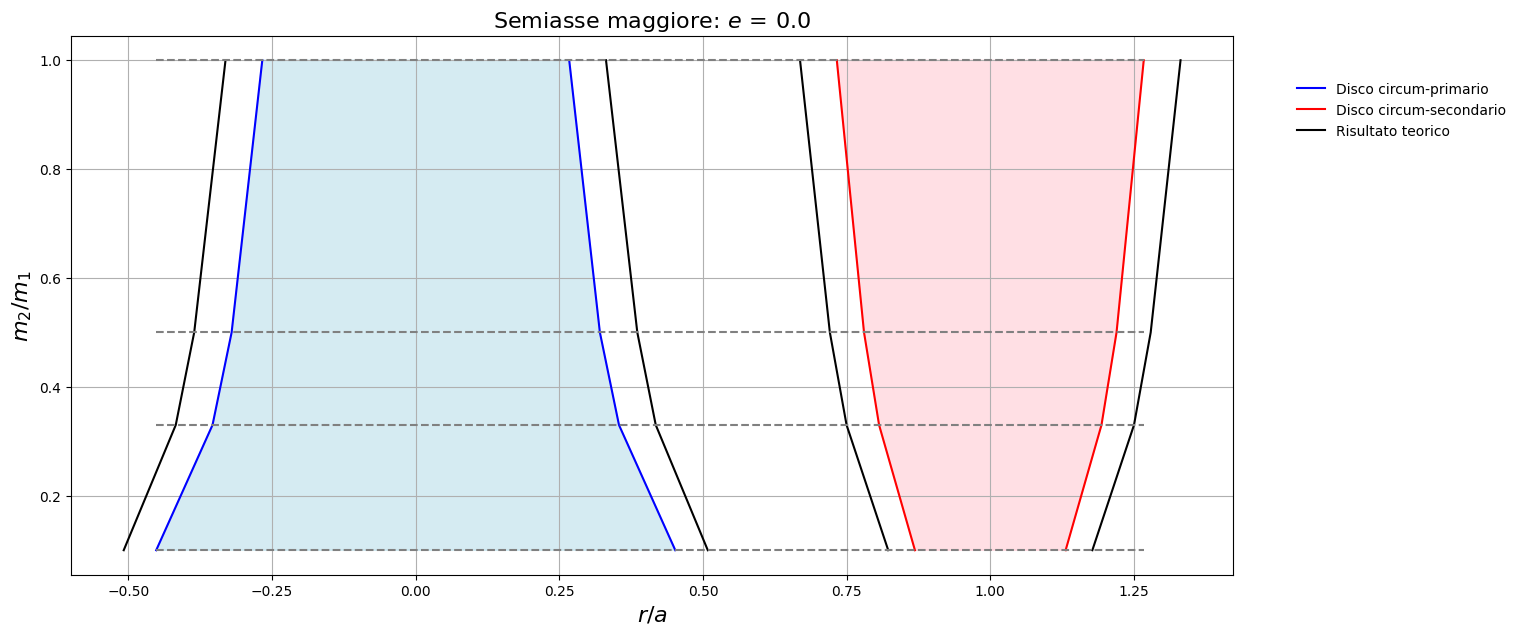
\includegraphics[width=\textwidth]{Immagini/Confronto/confax_A3_e0.png}
  \caption{Confronto fra modello teorico e valori numerici con: $\alpha\,=\,10^{-3}$, $e\,=\,0.0$. Notiamo che entrambe sia i dischi circum-primari che i dischi circum-secondari sono meno estesi delle predizioni della \ref{eq:tronc_disc}.}
  \label{fig:conf_ax30}
\end{figure}

\begin{figure}[H]
  \centering
  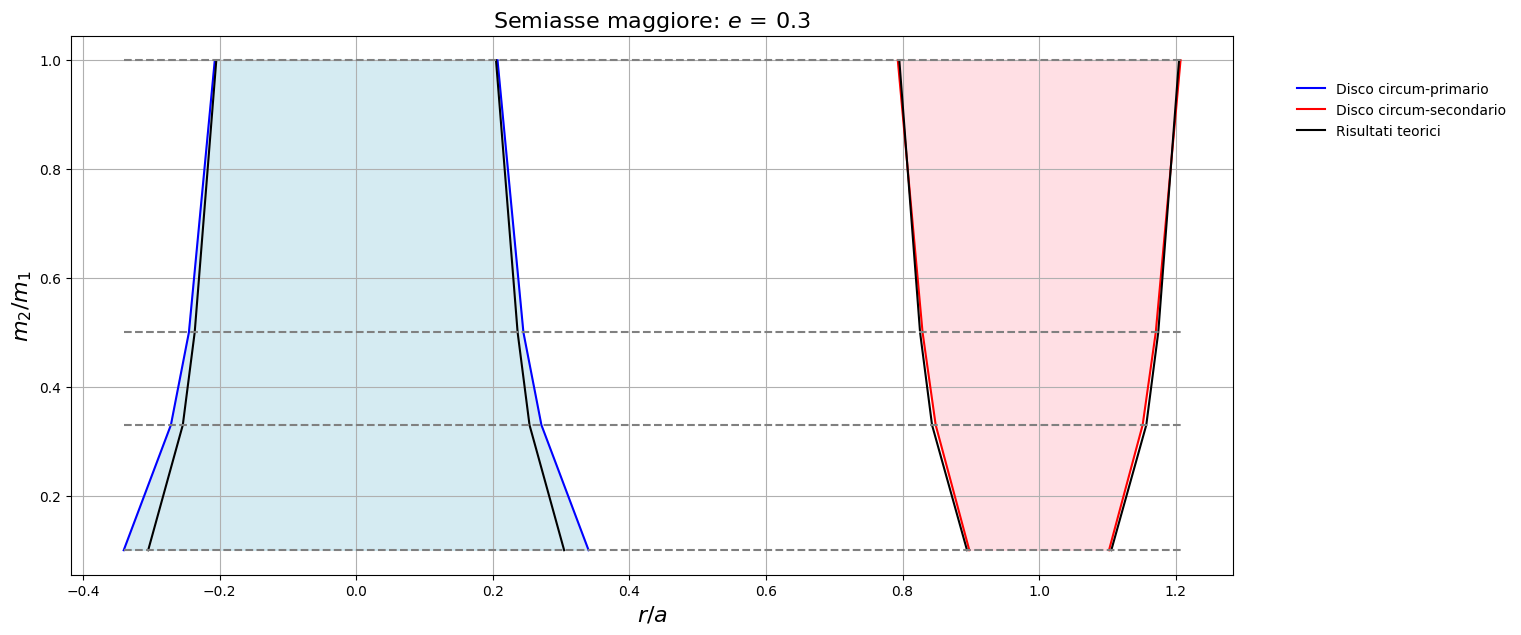
\includegraphics[width=\textwidth]{Immagini/Confronto/confax_A3_e3.png}
  \caption{Valori numerici e teorici per $\alpha\,=\,10^{-3}$, $e\,=\,0.3$. Il disco circum-primario risulta più esteso per bassi $m_2/m_1$.}
  \label{fig:conf_ax33}
\end{figure}

Come nel dischi caratterizzati da $\alpha\,=\,10^{-2}$, nel caso di binaria altamente eccentrica osserviamo un'elevata compatibilità fra valori numerici e teorici (vedi Figura \ref{fig:conf_ax36}).

\begin{figure}[H]
  \centering
  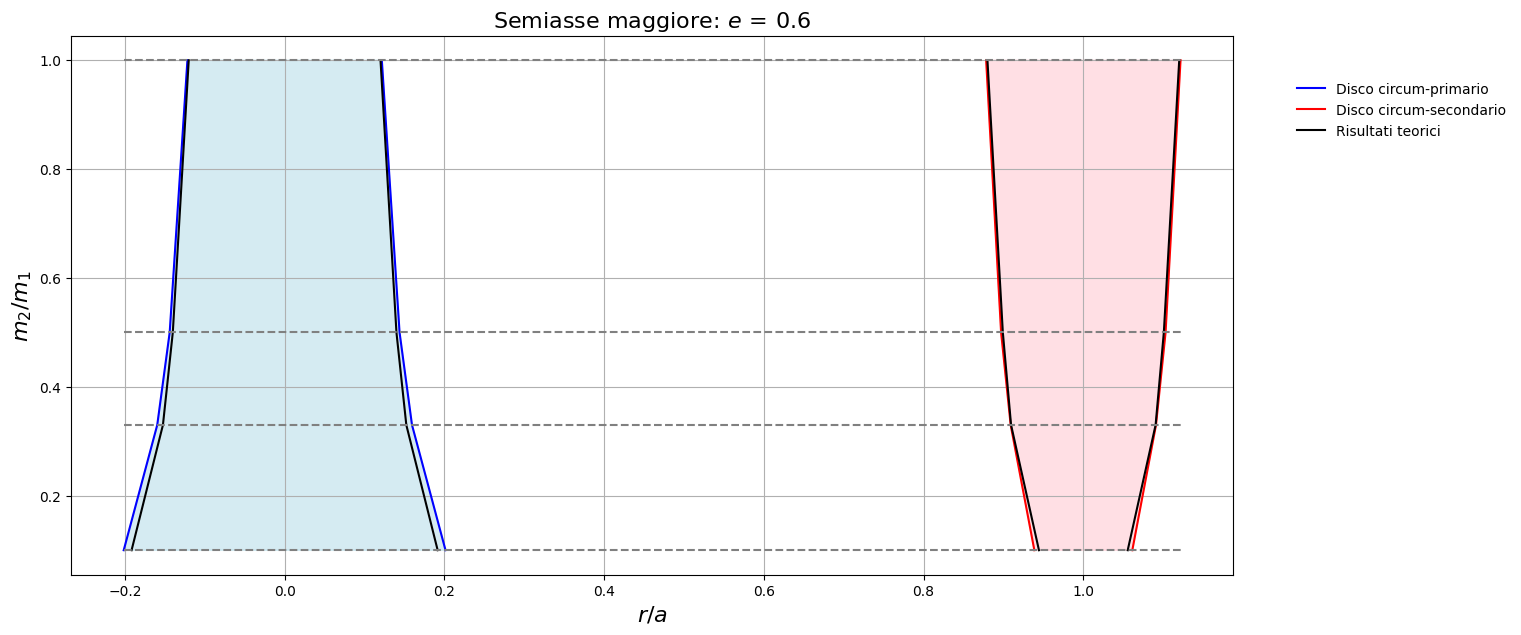
\includegraphics[width=\textwidth]{Immagini/Confronto/confax_A3_e6.png}
  \caption{Paragone fra valori numerici e teorici per dischi circumstellari facenti parte di un sistema ad elevata eccentricità. Il materiale orbitante ha $\alpha\,=\,10^{-3}$. Le due stime sono altamente compatibili per entrambi i dischi. }
  \label{fig:conf_ax36}
\end{figure}

\textbf{Viscosità minima}\\

Il materiale a viscosità minima è caratterizzato da $\alpha\,=\,10^{-4}$.
Come per gli altri due valori del parametro adimensionale $\alpha$ osserviamo che entrambi i dischi simulati sono di dimensioni inferiori rispetto alle predizioni (vedi Figura \ref{fig:conf_ax40}).

\begin{figure}[H]
  \centering
  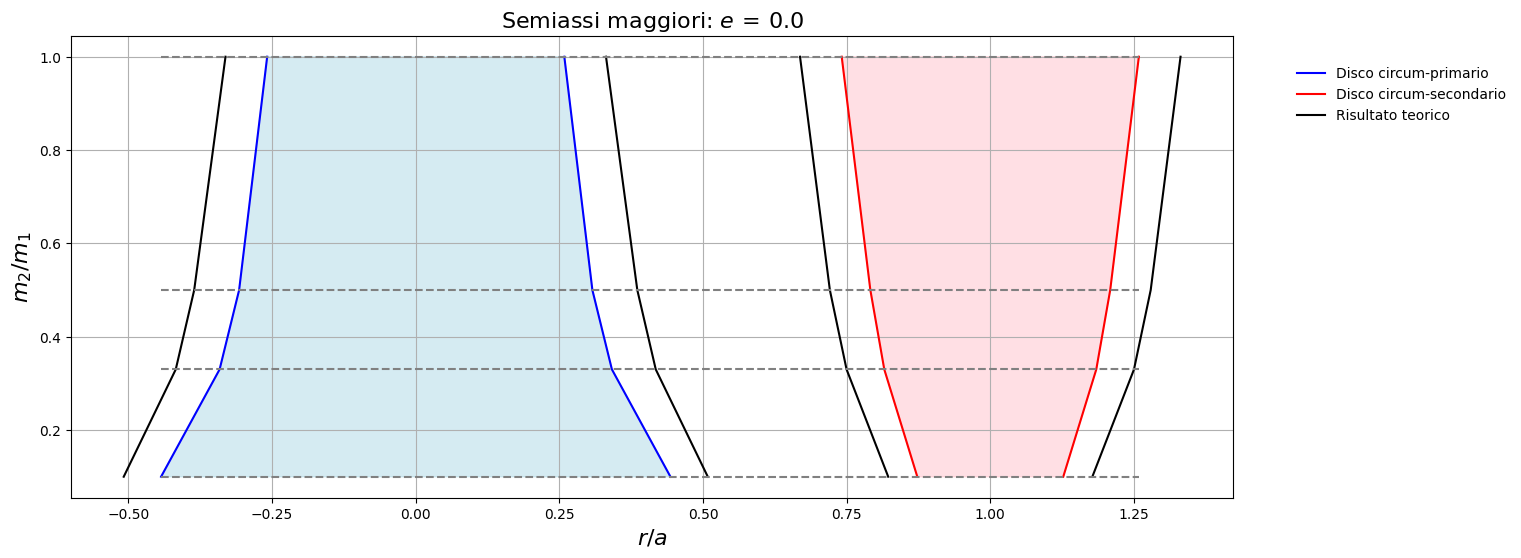
\includegraphics[width=\textwidth]{Immagini/Confronto/confax_A4_e0.png}
  \caption{Paragone fra dimensioni teoriche e numeriche dei dischi circumstellari con $\alpha\,=\,10^{-4}$ ed $e\,=\,0.0$. Sia i dischi circum-primari che quelli circum-secondari risultano più piccoli delle predizioni della \eqref{eq:tronc_disc}.}
  \label{fig:conf_ax40}
\end{figure}

I dischi in sistemi mediamente od altamente eccentrici presentano un buon accordo con il modello teorico, sebbene per entrambi i valori di $e$ il circum-primario simulato presenti una differente dipendenza da $m_2/m_1$, che comporta delle dimensioni maggiori per bassi valori di $q$. 

\begin{figure}[H]
  \centering
  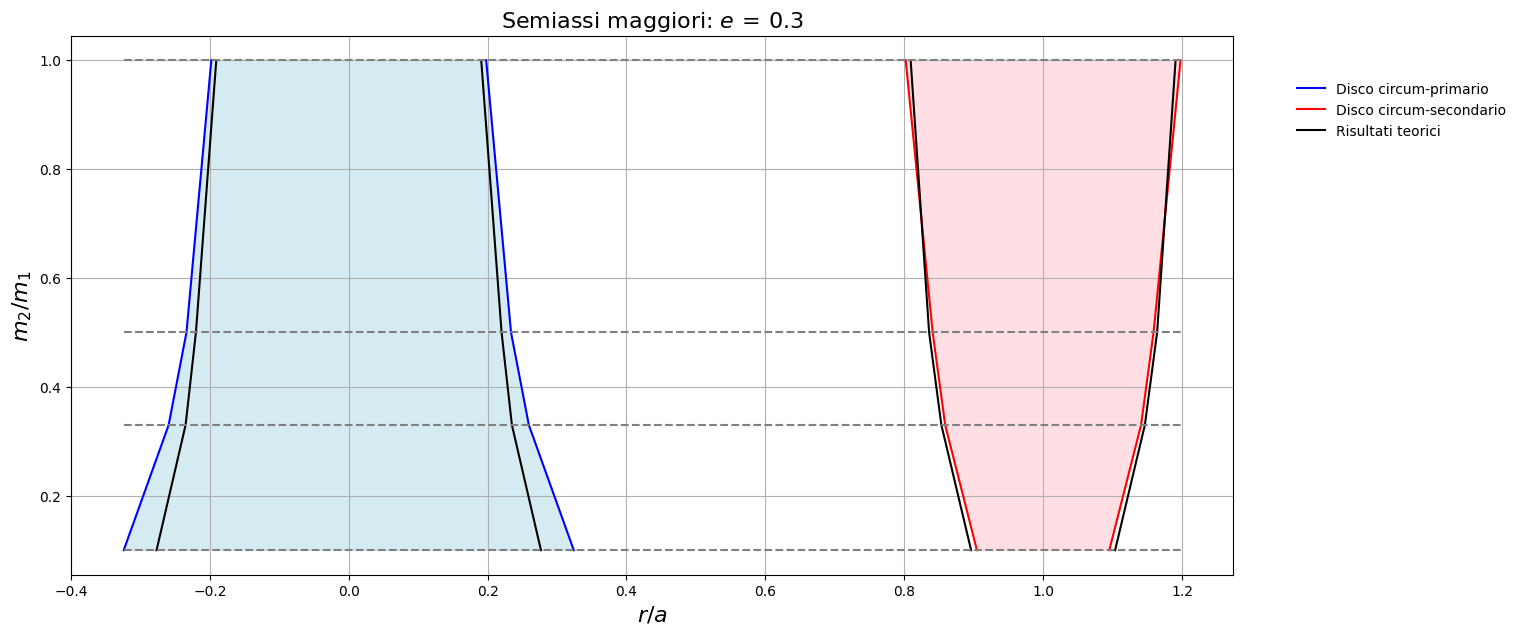
\includegraphics[width=\textwidth]{Immagini/Confronto/confax_A4_e3.png}
  \caption{Confronto fra modello teorico e risultati simulativi per dischi ospitati in un sistema binario mediamente eccentrico: $\alpha\,=\,10^{-4}$. Osserviamo che il disco circum-primario presenta delle dimensioni maggiori rispetto ai valori suggeriti dalla \eqref{eq:tronc_disc} per bassi valori di $m_2/m_1$.}
  \label{fig:conf_ax43}
\end{figure}

\begin{figure}[H]
  \centering
  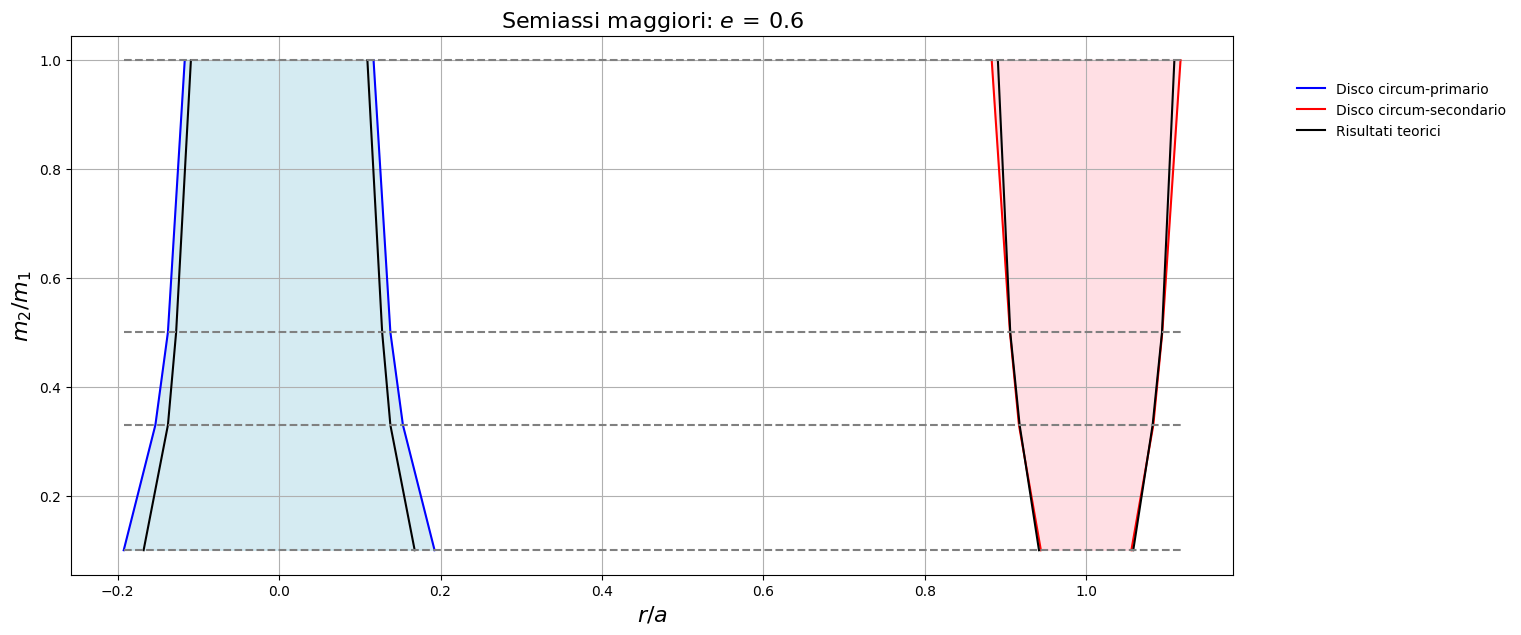
\includegraphics[width=\textwidth]{Immagini/Confronto/confax_A4_e6.png}
  \caption{In Figura sono riportate le dimensioni dei dischi circumstellari facenti parte di un sistema binario con $e\,=\,0.6$ e le predizioni teoriche: $\alpha\,=\,10^{-4}$. Notiamo che il disco circum-primario è più esteso di quanto suggerito dal modello proposto da \textcite{ManaraTronc2019} per piccoli $m_2/m_1$.}
  \label{fig:conf_ax46}
\end{figure}